\documentclass{article}
\usepackage[final]{neurips_2025}  % NEURIPS style (neurips_2025.sty is in paper_draft/)
\makeatletter\providecommand{\@trackname}{\@neuripsordinal\ Conference on Neural Information Processing Systems (NeurIPS \@neuripsyear).}\makeatother
\usepackage[hidelinks]{hyperref}  % REQUIRED: clickable links
\usepackage{booktabs}  % REQUIRED: professional tables
\usepackage{graphicx}
\usepackage{amsmath,amssymb}
\usepackage[utf8]{inputenc}
\usepackage[T1]{fontenc}
\usepackage{xspace}
\usepackage{enumitem}
\usepackage{subcaption}
\usepackage{multirow}
\usepackage{algorithm}
\usepackage[noend]{algpseudocode}

% Import command files
%%%%% MATH NOTATION MACROS %%%%%
% Standard math notation for academic papers
% Import with: %%%%% MATH NOTATION MACROS %%%%%
% Standard math notation for academic papers
% Import with: %%%%% MATH NOTATION MACROS %%%%%
% Standard math notation for academic papers
% Import with: \input{commands/math}

\usepackage{amsmath,amsfonts,bm}

%%%%%%%%%%%%%%%%%%%%%%%%%%%%%%%%%%%%%%%%%%%%%%%%%%%%%%%%%%%%%%%%%
% FIGURE AND SECTION REFERENCES
%%%%%%%%%%%%%%%%%%%%%%%%%%%%%%%%%%%%%%%%%%%%%%%%%%%%%%%%%%%%%%%%%

% Mark sections of captions for referring to divisions of figures
\newcommand{\figleft}{{\em (Left)}}
\newcommand{\figcenter}{{\em (Center)}}
\newcommand{\figright}{{\em (Right)}}
\newcommand{\figtop}{{\em (Top)}}
\newcommand{\figbottom}{{\em (Bottom)}}
\newcommand{\captiona}{{\em (a)}}
\newcommand{\captionb}{{\em (b)}}
\newcommand{\captionc}{{\em (c)}}
\newcommand{\captiond}{{\em (d)}}

% Figure references
\def\figref#1{figure~\ref{#1}}
\def\Figref#1{Figure~\ref{#1}}
\def\twofigref#1#2{figures \ref{#1} and \ref{#2}}
\def\quadfigref#1#2#3#4{figures \ref{#1}, \ref{#2}, \ref{#3} and \ref{#4}}

% Section references
\def\secref#1{section~\ref{#1}}
\def\Secref#1{Section~\ref{#1}}
\def\twosecrefs#1#2{sections \ref{#1} and \ref{#2}}
\def\secrefs#1#2#3{sections \ref{#1}, \ref{#2} and \ref{#3}}

% Equation references
\def\eqref#1{equation~\ref{#1}}
\def\Eqref#1{Equation~\ref{#1}}
\def\plaineqref#1{\ref{#1}}

% Algorithm references
\def\algref#1{algorithm~\ref{#1}}
\def\Algref#1{Algorithm~\ref{#1}}
\def\twoalgref#1#2{algorithms \ref{#1} and \ref{#2}}
\def\Twoalgref#1#2{Algorithms \ref{#1} and \ref{#2}}

% Table references
\def\tabref#1{table~\ref{#1}}
\def\Tabref#1{Table~\ref{#1}}

% Chapter references
\def\chapref#1{chapter~\ref{#1}}
\def\Chapref#1{Chapter~\ref{#1}}

%%%%%%%%%%%%%%%%%%%%%%%%%%%%%%%%%%%%%%%%%%%%%%%%%%%%%%%%%%%%%%%%%
% BASIC MATH DEFINITIONS
%%%%%%%%%%%%%%%%%%%%%%%%%%%%%%%%%%%%%%%%%%%%%%%%%%%%%%%%%%%%%%%%%

\def\ceil#1{\lceil #1 \rceil}
\def\floor#1{\lfloor #1 \rfloor}
\def\1{\bm{1}}
\def\eps{{\epsilon}}

% Common operators
\DeclareMathOperator*{\argmax}{arg\,max}
\DeclareMathOperator*{\argmin}{arg\,min}
\DeclareMathOperator{\sign}{sign}
\DeclareMathOperator{\Tr}{Tr}
\let\ab\allowbreak

%%%%%%%%%%%%%%%%%%%%%%%%%%%%%%%%%%%%%%%%%%%%%%%%%%%%%%%%%%%%%%%%%
% VECTORS (lowercase bold)
%%%%%%%%%%%%%%%%%%%%%%%%%%%%%%%%%%%%%%%%%%%%%%%%%%%%%%%%%%%%%%%%%

\def\vzero{{\bm{0}}}
\def\vone{{\bm{1}}}
\def\vmu{{\bm{\mu}}}
\def\vtheta{{\bm{\theta}}}
\def\va{{\bm{a}}}
\def\vb{{\bm{b}}}
\def\vc{{\bm{c}}}
\def\vd{{\bm{d}}}
\def\ve{{\bm{e}}}
\def\vf{{\bm{f}}}
\def\vg{{\bm{g}}}
\def\vh{{\bm{h}}}
\def\vi{{\bm{i}}}
\def\vj{{\bm{j}}}
\def\vk{{\bm{k}}}
\def\vl{{\bm{l}}}
\def\vm{{\bm{m}}}
\def\vn{{\bm{n}}}
\def\vo{{\bm{o}}}
\def\vp{{\bm{p}}}
\def\vq{{\bm{q}}}
\def\vr{{\bm{r}}}
\def\vs{{\bm{s}}}
\def\vt{{\bm{t}}}
\def\vu{{\bm{u}}}
\def\vv{{\bm{v}}}
\def\vw{{\bm{w}}}
\def\vx{{\bm{x}}}
\def\vy{{\bm{y}}}
\def\vz{{\bm{z}}}

%%%%%%%%%%%%%%%%%%%%%%%%%%%%%%%%%%%%%%%%%%%%%%%%%%%%%%%%%%%%%%%%%
% MATRICES (uppercase bold)
%%%%%%%%%%%%%%%%%%%%%%%%%%%%%%%%%%%%%%%%%%%%%%%%%%%%%%%%%%%%%%%%%

\def\mA{{\bm{A}}}
\def\mB{{\bm{B}}}
\def\mC{{\bm{C}}}
\def\mD{{\bm{D}}}
\def\mE{{\bm{E}}}
\def\mF{{\bm{F}}}
\def\mG{{\bm{G}}}
\def\mH{{\bm{H}}}
\def\mI{{\bm{I}}}
\def\mJ{{\bm{J}}}
\def\mK{{\bm{K}}}
\def\mL{{\bm{L}}}
\def\mM{{\bm{M}}}
\def\mN{{\bm{N}}}
\def\mO{{\bm{O}}}
\def\mP{{\bm{P}}}
\def\mQ{{\bm{Q}}}
\def\mR{{\bm{R}}}
\def\mS{{\bm{S}}}
\def\mT{{\bm{T}}}
\def\mU{{\bm{U}}}
\def\mV{{\bm{V}}}
\def\mW{{\bm{W}}}
\def\mX{{\bm{X}}}
\def\mY{{\bm{Y}}}
\def\mZ{{\bm{Z}}}
\def\mBeta{{\bm{\beta}}}
\def\mPhi{{\bm{\Phi}}}
\def\mLambda{{\bm{\Lambda}}}
\def\mSigma{{\bm{\Sigma}}}

%%%%%%%%%%%%%%%%%%%%%%%%%%%%%%%%%%%%%%%%%%%%%%%%%%%%%%%%%%%%%%%%%
% CALLIGRAPHIC (mathcal)
%%%%%%%%%%%%%%%%%%%%%%%%%%%%%%%%%%%%%%%%%%%%%%%%%%%%%%%%%%%%%%%%%

\def\gA{{\mathcal{A}}}
\def\gB{{\mathcal{B}}}
\def\gC{{\mathcal{C}}}
\def\gD{{\mathcal{D}}}
\def\gE{{\mathcal{E}}}
\def\gF{{\mathcal{F}}}
\def\gG{{\mathcal{G}}}
\def\gH{{\mathcal{H}}}
\def\gI{{\mathcal{I}}}
\def\gJ{{\mathcal{J}}}
\def\gK{{\mathcal{K}}}
\def\gL{{\mathcal{L}}}
\def\gM{{\mathcal{M}}}
\def\gN{{\mathcal{N}}}
\def\gO{{\mathcal{O}}}
\def\gP{{\mathcal{P}}}
\def\gQ{{\mathcal{Q}}}
\def\gR{{\mathcal{R}}}
\def\gS{{\mathcal{S}}}
\def\gT{{\mathcal{T}}}
\def\gU{{\mathcal{U}}}
\def\gV{{\mathcal{V}}}
\def\gW{{\mathcal{W}}}
\def\gX{{\mathcal{X}}}
\def\gY{{\mathcal{Y}}}
\def\gZ{{\mathcal{Z}}}

%%%%%%%%%%%%%%%%%%%%%%%%%%%%%%%%%%%%%%%%%%%%%%%%%%%%%%%%%%%%%%%%%
% SETS (blackboard bold)
%%%%%%%%%%%%%%%%%%%%%%%%%%%%%%%%%%%%%%%%%%%%%%%%%%%%%%%%%%%%%%%%%

\def\sA{{\mathbb{A}}}
\def\sB{{\mathbb{B}}}
\def\sC{{\mathbb{C}}}
\def\sD{{\mathbb{D}}}
\def\sF{{\mathbb{F}}}
\def\sG{{\mathbb{G}}}
\def\sH{{\mathbb{H}}}
\def\sI{{\mathbb{I}}}
\def\sJ{{\mathbb{J}}}
\def\sK{{\mathbb{K}}}
\def\sL{{\mathbb{L}}}
\def\sM{{\mathbb{M}}}
\def\sN{{\mathbb{N}}}
\def\sO{{\mathbb{O}}}
\def\sP{{\mathbb{P}}}
\def\sQ{{\mathbb{Q}}}
\def\sR{{\mathbb{R}}}
\def\sS{{\mathbb{S}}}
\def\sT{{\mathbb{T}}}
\def\sU{{\mathbb{U}}}
\def\sV{{\mathbb{V}}}
\def\sW{{\mathbb{W}}}
\def\sX{{\mathbb{X}}}
\def\sY{{\mathbb{Y}}}
\def\sZ{{\mathbb{Z}}}

%%%%%%%%%%%%%%%%%%%%%%%%%%%%%%%%%%%%%%%%%%%%%%%%%%%%%%%%%%%%%%%%%
% COMMON MATH SHORTCUTS
%%%%%%%%%%%%%%%%%%%%%%%%%%%%%%%%%%%%%%%%%%%%%%%%%%%%%%%%%%%%%%%%%

% Expectation and variance
\newcommand{\E}{\mathbb{E}}
\newcommand{\Var}{\mathrm{Var}}
\newcommand{\Cov}{\mathrm{Cov}}
\newcommand{\R}{\mathbb{R}}

% Datasets
\newcommand{\train}{\mathcal{D}}
\newcommand{\valid}{\mathcal{D_{\mathrm{valid}}}}
\newcommand{\test}{\mathcal{D_{\mathrm{test}}}}

% Distributions
\newcommand{\laplace}{\mathrm{Laplace}}
\newcommand{\Uniform}{\mathrm{Unif}}
\newcommand{\Normal}{\mathrm{Normal}}
\newcommand{\Categorical}{\mathrm{Categorical}}

% Common functions
\newcommand{\softmax}{\mathrm{softmax}}
\newcommand{\sigmoid}{\sigma}
\newcommand{\KL}{D_{\mathrm{KL}}}

% Norms
\newcommand{\normlzero}{L^0}
\newcommand{\normlone}{L^1}
\newcommand{\normltwo}{L^2}
\newcommand{\normlp}{L^p}
\newcommand{\normmax}{L^\infty}

%%%%%%%%%%%%%%%%%%%%%%%%%%%%%%%%%%%%%%%%%%%%%%%%%%%%%%%%%%%%%%%%%
% DEFINITIONS AND HIGHLIGHTING
%%%%%%%%%%%%%%%%%%%%%%%%%%%%%%%%%%%%%%%%%%%%%%%%%%%%%%%%%%%%%%%%%

% Highlight a newly defined term
\newcommand{\newterm}[1]{{\bf #1}}
\newcommand{\defn}[1]{\textbf{#1}}
\newcommand{\defeq}{\mathrel{\stackrel{\textnormal{\tiny def}}{=}}}


\usepackage{amsmath,amsfonts,bm}

%%%%%%%%%%%%%%%%%%%%%%%%%%%%%%%%%%%%%%%%%%%%%%%%%%%%%%%%%%%%%%%%%
% FIGURE AND SECTION REFERENCES
%%%%%%%%%%%%%%%%%%%%%%%%%%%%%%%%%%%%%%%%%%%%%%%%%%%%%%%%%%%%%%%%%

% Mark sections of captions for referring to divisions of figures
\newcommand{\figleft}{{\em (Left)}}
\newcommand{\figcenter}{{\em (Center)}}
\newcommand{\figright}{{\em (Right)}}
\newcommand{\figtop}{{\em (Top)}}
\newcommand{\figbottom}{{\em (Bottom)}}
\newcommand{\captiona}{{\em (a)}}
\newcommand{\captionb}{{\em (b)}}
\newcommand{\captionc}{{\em (c)}}
\newcommand{\captiond}{{\em (d)}}

% Figure references
\def\figref#1{figure~\ref{#1}}
\def\Figref#1{Figure~\ref{#1}}
\def\twofigref#1#2{figures \ref{#1} and \ref{#2}}
\def\quadfigref#1#2#3#4{figures \ref{#1}, \ref{#2}, \ref{#3} and \ref{#4}}

% Section references
\def\secref#1{section~\ref{#1}}
\def\Secref#1{Section~\ref{#1}}
\def\twosecrefs#1#2{sections \ref{#1} and \ref{#2}}
\def\secrefs#1#2#3{sections \ref{#1}, \ref{#2} and \ref{#3}}

% Equation references
\def\eqref#1{equation~\ref{#1}}
\def\Eqref#1{Equation~\ref{#1}}
\def\plaineqref#1{\ref{#1}}

% Algorithm references
\def\algref#1{algorithm~\ref{#1}}
\def\Algref#1{Algorithm~\ref{#1}}
\def\twoalgref#1#2{algorithms \ref{#1} and \ref{#2}}
\def\Twoalgref#1#2{Algorithms \ref{#1} and \ref{#2}}

% Table references
\def\tabref#1{table~\ref{#1}}
\def\Tabref#1{Table~\ref{#1}}

% Chapter references
\def\chapref#1{chapter~\ref{#1}}
\def\Chapref#1{Chapter~\ref{#1}}

%%%%%%%%%%%%%%%%%%%%%%%%%%%%%%%%%%%%%%%%%%%%%%%%%%%%%%%%%%%%%%%%%
% BASIC MATH DEFINITIONS
%%%%%%%%%%%%%%%%%%%%%%%%%%%%%%%%%%%%%%%%%%%%%%%%%%%%%%%%%%%%%%%%%

\def\ceil#1{\lceil #1 \rceil}
\def\floor#1{\lfloor #1 \rfloor}
\def\1{\bm{1}}
\def\eps{{\epsilon}}

% Common operators
\DeclareMathOperator*{\argmax}{arg\,max}
\DeclareMathOperator*{\argmin}{arg\,min}
\DeclareMathOperator{\sign}{sign}
\DeclareMathOperator{\Tr}{Tr}
\let\ab\allowbreak

%%%%%%%%%%%%%%%%%%%%%%%%%%%%%%%%%%%%%%%%%%%%%%%%%%%%%%%%%%%%%%%%%
% VECTORS (lowercase bold)
%%%%%%%%%%%%%%%%%%%%%%%%%%%%%%%%%%%%%%%%%%%%%%%%%%%%%%%%%%%%%%%%%

\def\vzero{{\bm{0}}}
\def\vone{{\bm{1}}}
\def\vmu{{\bm{\mu}}}
\def\vtheta{{\bm{\theta}}}
\def\va{{\bm{a}}}
\def\vb{{\bm{b}}}
\def\vc{{\bm{c}}}
\def\vd{{\bm{d}}}
\def\ve{{\bm{e}}}
\def\vf{{\bm{f}}}
\def\vg{{\bm{g}}}
\def\vh{{\bm{h}}}
\def\vi{{\bm{i}}}
\def\vj{{\bm{j}}}
\def\vk{{\bm{k}}}
\def\vl{{\bm{l}}}
\def\vm{{\bm{m}}}
\def\vn{{\bm{n}}}
\def\vo{{\bm{o}}}
\def\vp{{\bm{p}}}
\def\vq{{\bm{q}}}
\def\vr{{\bm{r}}}
\def\vs{{\bm{s}}}
\def\vt{{\bm{t}}}
\def\vu{{\bm{u}}}
\def\vv{{\bm{v}}}
\def\vw{{\bm{w}}}
\def\vx{{\bm{x}}}
\def\vy{{\bm{y}}}
\def\vz{{\bm{z}}}

%%%%%%%%%%%%%%%%%%%%%%%%%%%%%%%%%%%%%%%%%%%%%%%%%%%%%%%%%%%%%%%%%
% MATRICES (uppercase bold)
%%%%%%%%%%%%%%%%%%%%%%%%%%%%%%%%%%%%%%%%%%%%%%%%%%%%%%%%%%%%%%%%%

\def\mA{{\bm{A}}}
\def\mB{{\bm{B}}}
\def\mC{{\bm{C}}}
\def\mD{{\bm{D}}}
\def\mE{{\bm{E}}}
\def\mF{{\bm{F}}}
\def\mG{{\bm{G}}}
\def\mH{{\bm{H}}}
\def\mI{{\bm{I}}}
\def\mJ{{\bm{J}}}
\def\mK{{\bm{K}}}
\def\mL{{\bm{L}}}
\def\mM{{\bm{M}}}
\def\mN{{\bm{N}}}
\def\mO{{\bm{O}}}
\def\mP{{\bm{P}}}
\def\mQ{{\bm{Q}}}
\def\mR{{\bm{R}}}
\def\mS{{\bm{S}}}
\def\mT{{\bm{T}}}
\def\mU{{\bm{U}}}
\def\mV{{\bm{V}}}
\def\mW{{\bm{W}}}
\def\mX{{\bm{X}}}
\def\mY{{\bm{Y}}}
\def\mZ{{\bm{Z}}}
\def\mBeta{{\bm{\beta}}}
\def\mPhi{{\bm{\Phi}}}
\def\mLambda{{\bm{\Lambda}}}
\def\mSigma{{\bm{\Sigma}}}

%%%%%%%%%%%%%%%%%%%%%%%%%%%%%%%%%%%%%%%%%%%%%%%%%%%%%%%%%%%%%%%%%
% CALLIGRAPHIC (mathcal)
%%%%%%%%%%%%%%%%%%%%%%%%%%%%%%%%%%%%%%%%%%%%%%%%%%%%%%%%%%%%%%%%%

\def\gA{{\mathcal{A}}}
\def\gB{{\mathcal{B}}}
\def\gC{{\mathcal{C}}}
\def\gD{{\mathcal{D}}}
\def\gE{{\mathcal{E}}}
\def\gF{{\mathcal{F}}}
\def\gG{{\mathcal{G}}}
\def\gH{{\mathcal{H}}}
\def\gI{{\mathcal{I}}}
\def\gJ{{\mathcal{J}}}
\def\gK{{\mathcal{K}}}
\def\gL{{\mathcal{L}}}
\def\gM{{\mathcal{M}}}
\def\gN{{\mathcal{N}}}
\def\gO{{\mathcal{O}}}
\def\gP{{\mathcal{P}}}
\def\gQ{{\mathcal{Q}}}
\def\gR{{\mathcal{R}}}
\def\gS{{\mathcal{S}}}
\def\gT{{\mathcal{T}}}
\def\gU{{\mathcal{U}}}
\def\gV{{\mathcal{V}}}
\def\gW{{\mathcal{W}}}
\def\gX{{\mathcal{X}}}
\def\gY{{\mathcal{Y}}}
\def\gZ{{\mathcal{Z}}}

%%%%%%%%%%%%%%%%%%%%%%%%%%%%%%%%%%%%%%%%%%%%%%%%%%%%%%%%%%%%%%%%%
% SETS (blackboard bold)
%%%%%%%%%%%%%%%%%%%%%%%%%%%%%%%%%%%%%%%%%%%%%%%%%%%%%%%%%%%%%%%%%

\def\sA{{\mathbb{A}}}
\def\sB{{\mathbb{B}}}
\def\sC{{\mathbb{C}}}
\def\sD{{\mathbb{D}}}
\def\sF{{\mathbb{F}}}
\def\sG{{\mathbb{G}}}
\def\sH{{\mathbb{H}}}
\def\sI{{\mathbb{I}}}
\def\sJ{{\mathbb{J}}}
\def\sK{{\mathbb{K}}}
\def\sL{{\mathbb{L}}}
\def\sM{{\mathbb{M}}}
\def\sN{{\mathbb{N}}}
\def\sO{{\mathbb{O}}}
\def\sP{{\mathbb{P}}}
\def\sQ{{\mathbb{Q}}}
\def\sR{{\mathbb{R}}}
\def\sS{{\mathbb{S}}}
\def\sT{{\mathbb{T}}}
\def\sU{{\mathbb{U}}}
\def\sV{{\mathbb{V}}}
\def\sW{{\mathbb{W}}}
\def\sX{{\mathbb{X}}}
\def\sY{{\mathbb{Y}}}
\def\sZ{{\mathbb{Z}}}

%%%%%%%%%%%%%%%%%%%%%%%%%%%%%%%%%%%%%%%%%%%%%%%%%%%%%%%%%%%%%%%%%
% COMMON MATH SHORTCUTS
%%%%%%%%%%%%%%%%%%%%%%%%%%%%%%%%%%%%%%%%%%%%%%%%%%%%%%%%%%%%%%%%%

% Expectation and variance
\newcommand{\E}{\mathbb{E}}
\newcommand{\Var}{\mathrm{Var}}
\newcommand{\Cov}{\mathrm{Cov}}
\newcommand{\R}{\mathbb{R}}

% Datasets
\newcommand{\train}{\mathcal{D}}
\newcommand{\valid}{\mathcal{D_{\mathrm{valid}}}}
\newcommand{\test}{\mathcal{D_{\mathrm{test}}}}

% Distributions
\newcommand{\laplace}{\mathrm{Laplace}}
\newcommand{\Uniform}{\mathrm{Unif}}
\newcommand{\Normal}{\mathrm{Normal}}
\newcommand{\Categorical}{\mathrm{Categorical}}

% Common functions
\newcommand{\softmax}{\mathrm{softmax}}
\newcommand{\sigmoid}{\sigma}
\newcommand{\KL}{D_{\mathrm{KL}}}

% Norms
\newcommand{\normlzero}{L^0}
\newcommand{\normlone}{L^1}
\newcommand{\normltwo}{L^2}
\newcommand{\normlp}{L^p}
\newcommand{\normmax}{L^\infty}

%%%%%%%%%%%%%%%%%%%%%%%%%%%%%%%%%%%%%%%%%%%%%%%%%%%%%%%%%%%%%%%%%
% DEFINITIONS AND HIGHLIGHTING
%%%%%%%%%%%%%%%%%%%%%%%%%%%%%%%%%%%%%%%%%%%%%%%%%%%%%%%%%%%%%%%%%

% Highlight a newly defined term
\newcommand{\newterm}[1]{{\bf #1}}
\newcommand{\defn}[1]{\textbf{#1}}
\newcommand{\defeq}{\mathrel{\stackrel{\textnormal{\tiny def}}{=}}}


\usepackage{amsmath,amsfonts,bm}

%%%%%%%%%%%%%%%%%%%%%%%%%%%%%%%%%%%%%%%%%%%%%%%%%%%%%%%%%%%%%%%%%
% FIGURE AND SECTION REFERENCES
%%%%%%%%%%%%%%%%%%%%%%%%%%%%%%%%%%%%%%%%%%%%%%%%%%%%%%%%%%%%%%%%%

% Mark sections of captions for referring to divisions of figures
\newcommand{\figleft}{{\em (Left)}}
\newcommand{\figcenter}{{\em (Center)}}
\newcommand{\figright}{{\em (Right)}}
\newcommand{\figtop}{{\em (Top)}}
\newcommand{\figbottom}{{\em (Bottom)}}
\newcommand{\captiona}{{\em (a)}}
\newcommand{\captionb}{{\em (b)}}
\newcommand{\captionc}{{\em (c)}}
\newcommand{\captiond}{{\em (d)}}

% Figure references
\def\figref#1{figure~\ref{#1}}
\def\Figref#1{Figure~\ref{#1}}
\def\twofigref#1#2{figures \ref{#1} and \ref{#2}}
\def\quadfigref#1#2#3#4{figures \ref{#1}, \ref{#2}, \ref{#3} and \ref{#4}}

% Section references
\def\secref#1{section~\ref{#1}}
\def\Secref#1{Section~\ref{#1}}
\def\twosecrefs#1#2{sections \ref{#1} and \ref{#2}}
\def\secrefs#1#2#3{sections \ref{#1}, \ref{#2} and \ref{#3}}

% Equation references
\def\eqref#1{equation~\ref{#1}}
\def\Eqref#1{Equation~\ref{#1}}
\def\plaineqref#1{\ref{#1}}

% Algorithm references
\def\algref#1{algorithm~\ref{#1}}
\def\Algref#1{Algorithm~\ref{#1}}
\def\twoalgref#1#2{algorithms \ref{#1} and \ref{#2}}
\def\Twoalgref#1#2{Algorithms \ref{#1} and \ref{#2}}

% Table references
\def\tabref#1{table~\ref{#1}}
\def\Tabref#1{Table~\ref{#1}}

% Chapter references
\def\chapref#1{chapter~\ref{#1}}
\def\Chapref#1{Chapter~\ref{#1}}

%%%%%%%%%%%%%%%%%%%%%%%%%%%%%%%%%%%%%%%%%%%%%%%%%%%%%%%%%%%%%%%%%
% BASIC MATH DEFINITIONS
%%%%%%%%%%%%%%%%%%%%%%%%%%%%%%%%%%%%%%%%%%%%%%%%%%%%%%%%%%%%%%%%%

\def\ceil#1{\lceil #1 \rceil}
\def\floor#1{\lfloor #1 \rfloor}
\def\1{\bm{1}}
\def\eps{{\epsilon}}

% Common operators
\DeclareMathOperator*{\argmax}{arg\,max}
\DeclareMathOperator*{\argmin}{arg\,min}
\DeclareMathOperator{\sign}{sign}
\DeclareMathOperator{\Tr}{Tr}
\let\ab\allowbreak

%%%%%%%%%%%%%%%%%%%%%%%%%%%%%%%%%%%%%%%%%%%%%%%%%%%%%%%%%%%%%%%%%
% VECTORS (lowercase bold)
%%%%%%%%%%%%%%%%%%%%%%%%%%%%%%%%%%%%%%%%%%%%%%%%%%%%%%%%%%%%%%%%%

\def\vzero{{\bm{0}}}
\def\vone{{\bm{1}}}
\def\vmu{{\bm{\mu}}}
\def\vtheta{{\bm{\theta}}}
\def\va{{\bm{a}}}
\def\vb{{\bm{b}}}
\def\vc{{\bm{c}}}
\def\vd{{\bm{d}}}
\def\ve{{\bm{e}}}
\def\vf{{\bm{f}}}
\def\vg{{\bm{g}}}
\def\vh{{\bm{h}}}
\def\vi{{\bm{i}}}
\def\vj{{\bm{j}}}
\def\vk{{\bm{k}}}
\def\vl{{\bm{l}}}
\def\vm{{\bm{m}}}
\def\vn{{\bm{n}}}
\def\vo{{\bm{o}}}
\def\vp{{\bm{p}}}
\def\vq{{\bm{q}}}
\def\vr{{\bm{r}}}
\def\vs{{\bm{s}}}
\def\vt{{\bm{t}}}
\def\vu{{\bm{u}}}
\def\vv{{\bm{v}}}
\def\vw{{\bm{w}}}
\def\vx{{\bm{x}}}
\def\vy{{\bm{y}}}
\def\vz{{\bm{z}}}

%%%%%%%%%%%%%%%%%%%%%%%%%%%%%%%%%%%%%%%%%%%%%%%%%%%%%%%%%%%%%%%%%
% MATRICES (uppercase bold)
%%%%%%%%%%%%%%%%%%%%%%%%%%%%%%%%%%%%%%%%%%%%%%%%%%%%%%%%%%%%%%%%%

\def\mA{{\bm{A}}}
\def\mB{{\bm{B}}}
\def\mC{{\bm{C}}}
\def\mD{{\bm{D}}}
\def\mE{{\bm{E}}}
\def\mF{{\bm{F}}}
\def\mG{{\bm{G}}}
\def\mH{{\bm{H}}}
\def\mI{{\bm{I}}}
\def\mJ{{\bm{J}}}
\def\mK{{\bm{K}}}
\def\mL{{\bm{L}}}
\def\mM{{\bm{M}}}
\def\mN{{\bm{N}}}
\def\mO{{\bm{O}}}
\def\mP{{\bm{P}}}
\def\mQ{{\bm{Q}}}
\def\mR{{\bm{R}}}
\def\mS{{\bm{S}}}
\def\mT{{\bm{T}}}
\def\mU{{\bm{U}}}
\def\mV{{\bm{V}}}
\def\mW{{\bm{W}}}
\def\mX{{\bm{X}}}
\def\mY{{\bm{Y}}}
\def\mZ{{\bm{Z}}}
\def\mBeta{{\bm{\beta}}}
\def\mPhi{{\bm{\Phi}}}
\def\mLambda{{\bm{\Lambda}}}
\def\mSigma{{\bm{\Sigma}}}

%%%%%%%%%%%%%%%%%%%%%%%%%%%%%%%%%%%%%%%%%%%%%%%%%%%%%%%%%%%%%%%%%
% CALLIGRAPHIC (mathcal)
%%%%%%%%%%%%%%%%%%%%%%%%%%%%%%%%%%%%%%%%%%%%%%%%%%%%%%%%%%%%%%%%%

\def\gA{{\mathcal{A}}}
\def\gB{{\mathcal{B}}}
\def\gC{{\mathcal{C}}}
\def\gD{{\mathcal{D}}}
\def\gE{{\mathcal{E}}}
\def\gF{{\mathcal{F}}}
\def\gG{{\mathcal{G}}}
\def\gH{{\mathcal{H}}}
\def\gI{{\mathcal{I}}}
\def\gJ{{\mathcal{J}}}
\def\gK{{\mathcal{K}}}
\def\gL{{\mathcal{L}}}
\def\gM{{\mathcal{M}}}
\def\gN{{\mathcal{N}}}
\def\gO{{\mathcal{O}}}
\def\gP{{\mathcal{P}}}
\def\gQ{{\mathcal{Q}}}
\def\gR{{\mathcal{R}}}
\def\gS{{\mathcal{S}}}
\def\gT{{\mathcal{T}}}
\def\gU{{\mathcal{U}}}
\def\gV{{\mathcal{V}}}
\def\gW{{\mathcal{W}}}
\def\gX{{\mathcal{X}}}
\def\gY{{\mathcal{Y}}}
\def\gZ{{\mathcal{Z}}}

%%%%%%%%%%%%%%%%%%%%%%%%%%%%%%%%%%%%%%%%%%%%%%%%%%%%%%%%%%%%%%%%%
% SETS (blackboard bold)
%%%%%%%%%%%%%%%%%%%%%%%%%%%%%%%%%%%%%%%%%%%%%%%%%%%%%%%%%%%%%%%%%

\def\sA{{\mathbb{A}}}
\def\sB{{\mathbb{B}}}
\def\sC{{\mathbb{C}}}
\def\sD{{\mathbb{D}}}
\def\sF{{\mathbb{F}}}
\def\sG{{\mathbb{G}}}
\def\sH{{\mathbb{H}}}
\def\sI{{\mathbb{I}}}
\def\sJ{{\mathbb{J}}}
\def\sK{{\mathbb{K}}}
\def\sL{{\mathbb{L}}}
\def\sM{{\mathbb{M}}}
\def\sN{{\mathbb{N}}}
\def\sO{{\mathbb{O}}}
\def\sP{{\mathbb{P}}}
\def\sQ{{\mathbb{Q}}}
\def\sR{{\mathbb{R}}}
\def\sS{{\mathbb{S}}}
\def\sT{{\mathbb{T}}}
\def\sU{{\mathbb{U}}}
\def\sV{{\mathbb{V}}}
\def\sW{{\mathbb{W}}}
\def\sX{{\mathbb{X}}}
\def\sY{{\mathbb{Y}}}
\def\sZ{{\mathbb{Z}}}

%%%%%%%%%%%%%%%%%%%%%%%%%%%%%%%%%%%%%%%%%%%%%%%%%%%%%%%%%%%%%%%%%
% COMMON MATH SHORTCUTS
%%%%%%%%%%%%%%%%%%%%%%%%%%%%%%%%%%%%%%%%%%%%%%%%%%%%%%%%%%%%%%%%%

% Expectation and variance
\newcommand{\E}{\mathbb{E}}
\newcommand{\Var}{\mathrm{Var}}
\newcommand{\Cov}{\mathrm{Cov}}
\newcommand{\R}{\mathbb{R}}

% Datasets
\newcommand{\train}{\mathcal{D}}
\newcommand{\valid}{\mathcal{D_{\mathrm{valid}}}}
\newcommand{\test}{\mathcal{D_{\mathrm{test}}}}

% Distributions
\newcommand{\laplace}{\mathrm{Laplace}}
\newcommand{\Uniform}{\mathrm{Unif}}
\newcommand{\Normal}{\mathrm{Normal}}
\newcommand{\Categorical}{\mathrm{Categorical}}

% Common functions
\newcommand{\softmax}{\mathrm{softmax}}
\newcommand{\sigmoid}{\sigma}
\newcommand{\KL}{D_{\mathrm{KL}}}

% Norms
\newcommand{\normlzero}{L^0}
\newcommand{\normlone}{L^1}
\newcommand{\normltwo}{L^2}
\newcommand{\normlp}{L^p}
\newcommand{\normmax}{L^\infty}

%%%%%%%%%%%%%%%%%%%%%%%%%%%%%%%%%%%%%%%%%%%%%%%%%%%%%%%%%%%%%%%%%
% DEFINITIONS AND HIGHLIGHTING
%%%%%%%%%%%%%%%%%%%%%%%%%%%%%%%%%%%%%%%%%%%%%%%%%%%%%%%%%%%%%%%%%

% Highlight a newly defined term
\newcommand{\newterm}[1]{{\bf #1}}
\newcommand{\defn}[1]{\textbf{#1}}
\newcommand{\defeq}{\mathrel{\stackrel{\textnormal{\tiny def}}{=}}}

%%%%% GENERAL FORMATTING MACROS %%%%%
% General formatting and styling macros for academic papers
% Import with: %%%%% GENERAL FORMATTING MACROS %%%%%
% General formatting and styling macros for academic papers
% Import with: %%%%% GENERAL FORMATTING MACROS %%%%%
% General formatting and styling macros for academic papers
% Import with: \input{commands/general}

%%%%%%%%%%%%%%%%%%%%%%%%%%%%%%%%%%%%%%%%%%%%%%%%%%%%%%%%%%%%%%%%%
% PARAGRAPH AND TEXT FORMATTING
%%%%%%%%%%%%%%%%%%%%%%%%%%%%%%%%%%%%%%%%%%%%%%%%%%%%%%%%%%%%%%%%%

% Bold paragraph headers (use: \para{Header.} followed by text)
\newcommand{\para}[1]{\noindent \textbf{#1}}

% Cut content for space (content is hidden but preserved in source)
\newcommand{\cutforspace}[1]{}

% Response/rebuttal formatting for reviews
\newcommand{\response}[1]{\vspace{3pt}\hrule\vspace{3pt}\textbf{#1:}}

%%%%%%%%%%%%%%%%%%%%%%%%%%%%%%%%%%%%%%%%%%%%%%%%%%%%%%%%%%%%%%%%%
% RESULT HIGHLIGHTING
%%%%%%%%%%%%%%%%%%%%%%%%%%%%%%%%%%%%%%%%%%%%%%%%%%%%%%%%%%%%%%%%%

\usepackage{xcolor}
\usepackage{bm}

% Colors for result arrows
\definecolor{pastelgreen}{RGB}{50,205,50}

% Arrows for showing improvement/decline in results
\newcommand{\increase}{\textcolor{pastelgreen}{\bm{$\uparrow$}}}
\newcommand{\decrease}{\textcolor{red}{\bm{$\downarrow$}}}

% Phantom star for alignment in tables (use where no significance marker needed)
\newcommand{\pstar}{\phantom{*}}

%%%%%%%%%%%%%%%%%%%%%%%%%%%%%%%%%%%%%%%%%%%%%%%%%%%%%%%%%%%%%%%%%
% HIGHLIGHT BOXES
%%%%%%%%%%%%%%%%%%%%%%%%%%%%%%%%%%%%%%%%%%%%%%%%%%%%%%%%%%%%%%%%%

% Background colors for highlight boxes
\definecolor{aigold}{RGB}{244,210,1}
\definecolor{aigreen}{RGB}{213,245,227}
\definecolor{humanpurple}{RGB}{235,222,240}
\definecolor{aired}{RGB}{255,180,181}
\definecolor{mypurple}{RGB}{147,112,219}
\definecolor{myorange}{RGB}{255,165,0}
\definecolor{commentgray}{RGB}{86,101,115}
\definecolor{mygray}{RGB}{169,169,169}

% Highlight boxes for examples, quotes, etc.
\newcommand{\lightgreen}[1]{\fcolorbox{aigreen}{aigreen}{\parbox{\linewidth}{#1}}}
\newcommand{\lightred}[1]{\colorbox{aired}{\parbox{\linewidth}{#1}}}

%%%%%%%%%%%%%%%%%%%%%%%%%%%%%%%%%%%%%%%%%%%%%%%%%%%%%%%%%%%%%%%%%
% ALGORITHM STYLING
%%%%%%%%%%%%%%%%%%%%%%%%%%%%%%%%%%%%%%%%%%%%%%%%%%%%%%%%%%%%%%%%%

% Comment style for algorithms (triangleright marker)
\newcommand{\rightcomment}[1]{\(\triangleright\) {\small \it #1}}

% Equation comments
\newcommand{\eqcomment}[1]{\addtocounter{equation}{1}\tag*{\rightcomment{#1}\quad(\theequation)}}

% Algorithm formatting (requires algorithm and algpseudocode packages)
% \usepackage{algorithm}
% \usepackage[noend]{algpseudocode}

% Customize algorithm appearance
\renewcommand{\algorithmicindent}{9pt}
% \renewcommand\algorithmicdo{:}
% \renewcommand\algorithmicthen{:}

% Algorithm input/output
% \algnewcommand\algorithmicinput{{\bfseries Input:}}
% \algnewcommand\INPUT{\item[\algorithmicinput]}
% \algnewcommand\algorithmicoutput{{\bfseries Output:}}
% \algnewcommand\OUTPUT{\item[\algorithmicoutput]}

%%%%%%%%%%%%%%%%%%%%%%%%%%%%%%%%%%%%%%%%%%%%%%%%%%%%%%%%%%%%%%%%%
% CODE LISTINGS
%%%%%%%%%%%%%%%%%%%%%%%%%%%%%%%%%%%%%%%%%%%%%%%%%%%%%%%%%%%%%%%%%

\usepackage{listings}

\definecolor{codepurple}{RGB}{128,0,128}

\lstdefinestyle{datalogstyle}{
    basicstyle={\tt \scriptsize},
    xleftmargin={6pt},
    xrightmargin={6pt},
    columns=flexible,
    breakindent=0pt,
    breaklines=true,
    frame=tb,
    stepnumber=1,
    firstnumber=1,
    numberfirstline=true,
    tabsize=2,
    extendedchars=true,
    columns=fullflexible,
    keepspaces=true,
    escapeinside={@}{@},
    captionpos=b,
    commentstyle=\color{black!65},
    numberstyle=\tiny\color{black!65},
    stringstyle=\color{codepurple},
    breakatwhitespace=false,
    mathescape=true,
    numbersep=5pt,
    showspaces=false,
    showstringspaces=false,
    showtabs=false,
    aboveskip={0.8\baselineskip},
    belowskip={0.2\baselineskip},
}
\lstset{style=datalogstyle}

% Rename listings to "Example"
\renewcommand{\lstlistingname}{Example}

% Vertical dots for code continuation
\newcommand{\progvdots}{\\[-4pt]$\vdots$}

%%%%%%%%%%%%%%%%%%%%%%%%%%%%%%%%%%%%%%%%%%%%%%%%%%%%%%%%%%%%%%%%%
% AUTHOR COMMENT SYSTEM
%%%%%%%%%%%%%%%%%%%%%%%%%%%%%%%%%%%%%%%%%%%%%%%%%%%%%%%%%%%%%%%%%

% Toggle to hide/show comments (uncomment \hidecommentstrue to hide)
\newif\ifhidecomments
% \hidecommentstrue

% Define author comments (add your own authors here)
% Each author gets a unique color
\ifhidecomments
    % Hidden mode - comments are invisible
    \newcommand{\authorone}[1]{}
    \newcommand{\authortwo}[1]{}
    \newcommand{\authorthree}[1]{}
\else
    % Visible mode - comments shown in color
    \newcommand{\authorone}[1]{\textcolor{blue}{[\textsc{AuthorOne}: #1]}}
    \newcommand{\authortwo}[1]{\textcolor{green!70!blue}{[\textsc{AuthorTwo}: #1]}}
    \newcommand{\authorthree}[1]{\textcolor{magenta!80!brown}{[\textsc{AuthorThree}: #1]}}
\fi

% Generic fixme/todo command
\newcommand{\fixme}[1]{\textcolor{red}{[FIXME: #1]}}

%%%%%%%%%%%%%%%%%%%%%%%%%%%%%%%%%%%%%%%%%%%%%%%%%%%%%%%%%%%%%%%%%
% SPACING CONFIGURATION
%%%%%%%%%%%%%%%%%%%%%%%%%%%%%%%%%%%%%%%%%%%%%%%%%%%%%%%%%%%%%%%%%

% Tight spacing for figures and tables (adjust as needed)
% \captionsetup[subfigure]{aboveskip=2pt,belowskip=2pt}
% \captionsetup[table]{aboveskip=4pt,belowskip=4pt}
% \captionsetup[figure]{aboveskip=4pt,belowskip=4pt}
% \setlength{\dbltextfloatsep}{11pt}
% \setlength{\dblfloatsep}{11pt}
% \setlength{\floatsep}{11pt}
% \setlength{\textfloatsep}{11pt}

%%%%%%%%%%%%%%%%%%%%%%%%%%%%%%%%%%%%%%%%%%%%%%%%%%%%%%%%%%%%%%%%%
% MISCELLANEOUS
%%%%%%%%%%%%%%%%%%%%%%%%%%%%%%%%%%%%%%%%%%%%%%%%%%%%%%%%%%%%%%%%%

% Ordinals
\renewcommand{\th}{\textsuperscript{th}\xspace}

% Special tokens
\newcommand{\bos}{\textsc{bos}\xspace}
\newcommand{\eos}{\textsc{eos}\xspace}

% Inverse notation
\newcommand{\inv}[1]{#1^{\scriptscriptstyle-\!1}}


%%%%%%%%%%%%%%%%%%%%%%%%%%%%%%%%%%%%%%%%%%%%%%%%%%%%%%%%%%%%%%%%%
% PARAGRAPH AND TEXT FORMATTING
%%%%%%%%%%%%%%%%%%%%%%%%%%%%%%%%%%%%%%%%%%%%%%%%%%%%%%%%%%%%%%%%%

% Bold paragraph headers (use: \para{Header.} followed by text)
\newcommand{\para}[1]{\noindent \textbf{#1}}

% Cut content for space (content is hidden but preserved in source)
\newcommand{\cutforspace}[1]{}

% Response/rebuttal formatting for reviews
\newcommand{\response}[1]{\vspace{3pt}\hrule\vspace{3pt}\textbf{#1:}}

%%%%%%%%%%%%%%%%%%%%%%%%%%%%%%%%%%%%%%%%%%%%%%%%%%%%%%%%%%%%%%%%%
% RESULT HIGHLIGHTING
%%%%%%%%%%%%%%%%%%%%%%%%%%%%%%%%%%%%%%%%%%%%%%%%%%%%%%%%%%%%%%%%%

\usepackage{xcolor}
\usepackage{bm}

% Colors for result arrows
\definecolor{pastelgreen}{RGB}{50,205,50}

% Arrows for showing improvement/decline in results
\newcommand{\increase}{\textcolor{pastelgreen}{\bm{$\uparrow$}}}
\newcommand{\decrease}{\textcolor{red}{\bm{$\downarrow$}}}

% Phantom star for alignment in tables (use where no significance marker needed)
\newcommand{\pstar}{\phantom{*}}

%%%%%%%%%%%%%%%%%%%%%%%%%%%%%%%%%%%%%%%%%%%%%%%%%%%%%%%%%%%%%%%%%
% HIGHLIGHT BOXES
%%%%%%%%%%%%%%%%%%%%%%%%%%%%%%%%%%%%%%%%%%%%%%%%%%%%%%%%%%%%%%%%%

% Background colors for highlight boxes
\definecolor{aigold}{RGB}{244,210,1}
\definecolor{aigreen}{RGB}{213,245,227}
\definecolor{humanpurple}{RGB}{235,222,240}
\definecolor{aired}{RGB}{255,180,181}
\definecolor{mypurple}{RGB}{147,112,219}
\definecolor{myorange}{RGB}{255,165,0}
\definecolor{commentgray}{RGB}{86,101,115}
\definecolor{mygray}{RGB}{169,169,169}

% Highlight boxes for examples, quotes, etc.
\newcommand{\lightgreen}[1]{\fcolorbox{aigreen}{aigreen}{\parbox{\linewidth}{#1}}}
\newcommand{\lightred}[1]{\colorbox{aired}{\parbox{\linewidth}{#1}}}

%%%%%%%%%%%%%%%%%%%%%%%%%%%%%%%%%%%%%%%%%%%%%%%%%%%%%%%%%%%%%%%%%
% ALGORITHM STYLING
%%%%%%%%%%%%%%%%%%%%%%%%%%%%%%%%%%%%%%%%%%%%%%%%%%%%%%%%%%%%%%%%%

% Comment style for algorithms (triangleright marker)
\newcommand{\rightcomment}[1]{\(\triangleright\) {\small \it #1}}

% Equation comments
\newcommand{\eqcomment}[1]{\addtocounter{equation}{1}\tag*{\rightcomment{#1}\quad(\theequation)}}

% Algorithm formatting (requires algorithm and algpseudocode packages)
% \usepackage{algorithm}
% \usepackage[noend]{algpseudocode}

% Customize algorithm appearance
\renewcommand{\algorithmicindent}{9pt}
% \renewcommand\algorithmicdo{:}
% \renewcommand\algorithmicthen{:}

% Algorithm input/output
% \algnewcommand\algorithmicinput{{\bfseries Input:}}
% \algnewcommand\INPUT{\item[\algorithmicinput]}
% \algnewcommand\algorithmicoutput{{\bfseries Output:}}
% \algnewcommand\OUTPUT{\item[\algorithmicoutput]}

%%%%%%%%%%%%%%%%%%%%%%%%%%%%%%%%%%%%%%%%%%%%%%%%%%%%%%%%%%%%%%%%%
% CODE LISTINGS
%%%%%%%%%%%%%%%%%%%%%%%%%%%%%%%%%%%%%%%%%%%%%%%%%%%%%%%%%%%%%%%%%

\usepackage{listings}

\definecolor{codepurple}{RGB}{128,0,128}

\lstdefinestyle{datalogstyle}{
    basicstyle={\tt \scriptsize},
    xleftmargin={6pt},
    xrightmargin={6pt},
    columns=flexible,
    breakindent=0pt,
    breaklines=true,
    frame=tb,
    stepnumber=1,
    firstnumber=1,
    numberfirstline=true,
    tabsize=2,
    extendedchars=true,
    columns=fullflexible,
    keepspaces=true,
    escapeinside={@}{@},
    captionpos=b,
    commentstyle=\color{black!65},
    numberstyle=\tiny\color{black!65},
    stringstyle=\color{codepurple},
    breakatwhitespace=false,
    mathescape=true,
    numbersep=5pt,
    showspaces=false,
    showstringspaces=false,
    showtabs=false,
    aboveskip={0.8\baselineskip},
    belowskip={0.2\baselineskip},
}
\lstset{style=datalogstyle}

% Rename listings to "Example"
\renewcommand{\lstlistingname}{Example}

% Vertical dots for code continuation
\newcommand{\progvdots}{\\[-4pt]$\vdots$}

%%%%%%%%%%%%%%%%%%%%%%%%%%%%%%%%%%%%%%%%%%%%%%%%%%%%%%%%%%%%%%%%%
% AUTHOR COMMENT SYSTEM
%%%%%%%%%%%%%%%%%%%%%%%%%%%%%%%%%%%%%%%%%%%%%%%%%%%%%%%%%%%%%%%%%

% Toggle to hide/show comments (uncomment \hidecommentstrue to hide)
\newif\ifhidecomments
% \hidecommentstrue

% Define author comments (add your own authors here)
% Each author gets a unique color
\ifhidecomments
    % Hidden mode - comments are invisible
    \newcommand{\authorone}[1]{}
    \newcommand{\authortwo}[1]{}
    \newcommand{\authorthree}[1]{}
\else
    % Visible mode - comments shown in color
    \newcommand{\authorone}[1]{\textcolor{blue}{[\textsc{AuthorOne}: #1]}}
    \newcommand{\authortwo}[1]{\textcolor{green!70!blue}{[\textsc{AuthorTwo}: #1]}}
    \newcommand{\authorthree}[1]{\textcolor{magenta!80!brown}{[\textsc{AuthorThree}: #1]}}
\fi

% Generic fixme/todo command
\newcommand{\fixme}[1]{\textcolor{red}{[FIXME: #1]}}

%%%%%%%%%%%%%%%%%%%%%%%%%%%%%%%%%%%%%%%%%%%%%%%%%%%%%%%%%%%%%%%%%
% SPACING CONFIGURATION
%%%%%%%%%%%%%%%%%%%%%%%%%%%%%%%%%%%%%%%%%%%%%%%%%%%%%%%%%%%%%%%%%

% Tight spacing for figures and tables (adjust as needed)
% \captionsetup[subfigure]{aboveskip=2pt,belowskip=2pt}
% \captionsetup[table]{aboveskip=4pt,belowskip=4pt}
% \captionsetup[figure]{aboveskip=4pt,belowskip=4pt}
% \setlength{\dbltextfloatsep}{11pt}
% \setlength{\dblfloatsep}{11pt}
% \setlength{\floatsep}{11pt}
% \setlength{\textfloatsep}{11pt}

%%%%%%%%%%%%%%%%%%%%%%%%%%%%%%%%%%%%%%%%%%%%%%%%%%%%%%%%%%%%%%%%%
% MISCELLANEOUS
%%%%%%%%%%%%%%%%%%%%%%%%%%%%%%%%%%%%%%%%%%%%%%%%%%%%%%%%%%%%%%%%%

% Ordinals
\renewcommand{\th}{\textsuperscript{th}\xspace}

% Special tokens
\newcommand{\bos}{\textsc{bos}\xspace}
\newcommand{\eos}{\textsc{eos}\xspace}

% Inverse notation
\newcommand{\inv}[1]{#1^{\scriptscriptstyle-\!1}}


%%%%%%%%%%%%%%%%%%%%%%%%%%%%%%%%%%%%%%%%%%%%%%%%%%%%%%%%%%%%%%%%%
% PARAGRAPH AND TEXT FORMATTING
%%%%%%%%%%%%%%%%%%%%%%%%%%%%%%%%%%%%%%%%%%%%%%%%%%%%%%%%%%%%%%%%%

% Bold paragraph headers (use: \para{Header.} followed by text)
\newcommand{\para}[1]{\noindent \textbf{#1}}

% Cut content for space (content is hidden but preserved in source)
\newcommand{\cutforspace}[1]{}

% Response/rebuttal formatting for reviews
\newcommand{\response}[1]{\vspace{3pt}\hrule\vspace{3pt}\textbf{#1:}}

%%%%%%%%%%%%%%%%%%%%%%%%%%%%%%%%%%%%%%%%%%%%%%%%%%%%%%%%%%%%%%%%%
% RESULT HIGHLIGHTING
%%%%%%%%%%%%%%%%%%%%%%%%%%%%%%%%%%%%%%%%%%%%%%%%%%%%%%%%%%%%%%%%%

\usepackage{xcolor}
\usepackage{bm}

% Colors for result arrows
\definecolor{pastelgreen}{RGB}{50,205,50}

% Arrows for showing improvement/decline in results
\newcommand{\increase}{\textcolor{pastelgreen}{\bm{$\uparrow$}}}
\newcommand{\decrease}{\textcolor{red}{\bm{$\downarrow$}}}

% Phantom star for alignment in tables (use where no significance marker needed)
\newcommand{\pstar}{\phantom{*}}

%%%%%%%%%%%%%%%%%%%%%%%%%%%%%%%%%%%%%%%%%%%%%%%%%%%%%%%%%%%%%%%%%
% HIGHLIGHT BOXES
%%%%%%%%%%%%%%%%%%%%%%%%%%%%%%%%%%%%%%%%%%%%%%%%%%%%%%%%%%%%%%%%%

% Background colors for highlight boxes
\definecolor{aigold}{RGB}{244,210,1}
\definecolor{aigreen}{RGB}{213,245,227}
\definecolor{humanpurple}{RGB}{235,222,240}
\definecolor{aired}{RGB}{255,180,181}
\definecolor{mypurple}{RGB}{147,112,219}
\definecolor{myorange}{RGB}{255,165,0}
\definecolor{commentgray}{RGB}{86,101,115}
\definecolor{mygray}{RGB}{169,169,169}

% Highlight boxes for examples, quotes, etc.
\newcommand{\lightgreen}[1]{\fcolorbox{aigreen}{aigreen}{\parbox{\linewidth}{#1}}}
\newcommand{\lightred}[1]{\colorbox{aired}{\parbox{\linewidth}{#1}}}

%%%%%%%%%%%%%%%%%%%%%%%%%%%%%%%%%%%%%%%%%%%%%%%%%%%%%%%%%%%%%%%%%
% ALGORITHM STYLING
%%%%%%%%%%%%%%%%%%%%%%%%%%%%%%%%%%%%%%%%%%%%%%%%%%%%%%%%%%%%%%%%%

% Comment style for algorithms (triangleright marker)
\newcommand{\rightcomment}[1]{\(\triangleright\) {\small \it #1}}

% Equation comments
\newcommand{\eqcomment}[1]{\addtocounter{equation}{1}\tag*{\rightcomment{#1}\quad(\theequation)}}

% Algorithm formatting (requires algorithm and algpseudocode packages)
% \usepackage{algorithm}
% \usepackage[noend]{algpseudocode}

% Customize algorithm appearance
\renewcommand{\algorithmicindent}{9pt}
% \renewcommand\algorithmicdo{:}
% \renewcommand\algorithmicthen{:}

% Algorithm input/output
% \algnewcommand\algorithmicinput{{\bfseries Input:}}
% \algnewcommand\INPUT{\item[\algorithmicinput]}
% \algnewcommand\algorithmicoutput{{\bfseries Output:}}
% \algnewcommand\OUTPUT{\item[\algorithmicoutput]}

%%%%%%%%%%%%%%%%%%%%%%%%%%%%%%%%%%%%%%%%%%%%%%%%%%%%%%%%%%%%%%%%%
% CODE LISTINGS
%%%%%%%%%%%%%%%%%%%%%%%%%%%%%%%%%%%%%%%%%%%%%%%%%%%%%%%%%%%%%%%%%

\usepackage{listings}

\definecolor{codepurple}{RGB}{128,0,128}

\lstdefinestyle{datalogstyle}{
    basicstyle={\tt \scriptsize},
    xleftmargin={6pt},
    xrightmargin={6pt},
    columns=flexible,
    breakindent=0pt,
    breaklines=true,
    frame=tb,
    stepnumber=1,
    firstnumber=1,
    numberfirstline=true,
    tabsize=2,
    extendedchars=true,
    columns=fullflexible,
    keepspaces=true,
    escapeinside={@}{@},
    captionpos=b,
    commentstyle=\color{black!65},
    numberstyle=\tiny\color{black!65},
    stringstyle=\color{codepurple},
    breakatwhitespace=false,
    mathescape=true,
    numbersep=5pt,
    showspaces=false,
    showstringspaces=false,
    showtabs=false,
    aboveskip={0.8\baselineskip},
    belowskip={0.2\baselineskip},
}
\lstset{style=datalogstyle}

% Rename listings to "Example"
\renewcommand{\lstlistingname}{Example}

% Vertical dots for code continuation
\newcommand{\progvdots}{\\[-4pt]$\vdots$}

%%%%%%%%%%%%%%%%%%%%%%%%%%%%%%%%%%%%%%%%%%%%%%%%%%%%%%%%%%%%%%%%%
% AUTHOR COMMENT SYSTEM
%%%%%%%%%%%%%%%%%%%%%%%%%%%%%%%%%%%%%%%%%%%%%%%%%%%%%%%%%%%%%%%%%

% Toggle to hide/show comments (uncomment \hidecommentstrue to hide)
\newif\ifhidecomments
% \hidecommentstrue

% Define author comments (add your own authors here)
% Each author gets a unique color
\ifhidecomments
    % Hidden mode - comments are invisible
    \newcommand{\authorone}[1]{}
    \newcommand{\authortwo}[1]{}
    \newcommand{\authorthree}[1]{}
\else
    % Visible mode - comments shown in color
    \newcommand{\authorone}[1]{\textcolor{blue}{[\textsc{AuthorOne}: #1]}}
    \newcommand{\authortwo}[1]{\textcolor{green!70!blue}{[\textsc{AuthorTwo}: #1]}}
    \newcommand{\authorthree}[1]{\textcolor{magenta!80!brown}{[\textsc{AuthorThree}: #1]}}
\fi

% Generic fixme/todo command
\newcommand{\fixme}[1]{\textcolor{red}{[FIXME: #1]}}

%%%%%%%%%%%%%%%%%%%%%%%%%%%%%%%%%%%%%%%%%%%%%%%%%%%%%%%%%%%%%%%%%
% SPACING CONFIGURATION
%%%%%%%%%%%%%%%%%%%%%%%%%%%%%%%%%%%%%%%%%%%%%%%%%%%%%%%%%%%%%%%%%

% Tight spacing for figures and tables (adjust as needed)
% \captionsetup[subfigure]{aboveskip=2pt,belowskip=2pt}
% \captionsetup[table]{aboveskip=4pt,belowskip=4pt}
% \captionsetup[figure]{aboveskip=4pt,belowskip=4pt}
% \setlength{\dbltextfloatsep}{11pt}
% \setlength{\dblfloatsep}{11pt}
% \setlength{\floatsep}{11pt}
% \setlength{\textfloatsep}{11pt}

%%%%%%%%%%%%%%%%%%%%%%%%%%%%%%%%%%%%%%%%%%%%%%%%%%%%%%%%%%%%%%%%%
% MISCELLANEOUS
%%%%%%%%%%%%%%%%%%%%%%%%%%%%%%%%%%%%%%%%%%%%%%%%%%%%%%%%%%%%%%%%%

% Ordinals
\renewcommand{\th}{\textsuperscript{th}\xspace}

% Special tokens
\newcommand{\bos}{\textsc{bos}\xspace}
\newcommand{\eos}{\textsc{eos}\xspace}

% Inverse notation
\newcommand{\inv}[1]{#1^{\scriptscriptstyle-\!1}}

%%%%% PROJECT-SPECIFIC MACROS %%%%%
\usepackage{xspace}

% Metric names
\newcommand{\pres}{kNN@10 preservation\xspace}
\newcommand{\knn}{\textsc{kNN}\xspace}
\newcommand{\cka}{\textsc{CKA}\xspace}
\newcommand{\isoscore}{\textsc{IsoScore}\xspace}
\newcommand{\gk}{\textsc{GK}\xspace}

% Dataset names
\newcommand{\wikitext}{\textsc{WikiText-103}\xspace}
\newcommand{\mmlu}{\textsc{MMLU}\xspace}
\newcommand{\arce}{\textsc{ARC-Easy}\xspace}
\newcommand{\asclepius}{\textsc{Asclepius}\xspace}
\newcommand{\codeparrot}{\textsc{CodeParrot}\xspace}

% Model names
\newcommand{\qwenS}{Qwen2.5-0.5B\xspace}
\newcommand{\qwenM}{Qwen2.5-1.5B\xspace}
\newcommand{\qwenL}{Qwen2.5-3B\xspace}
\newcommand{\pythiaS}{Pythia-160M\xspace}
\newcommand{\pythiaM}{Pythia-410M\xspace}

% Abbreviations
\newcommand{\ie}{i.e.,\xspace}
\newcommand{\eg}{e.g.,\xspace}
\newcommand{\versus}{vs.\xspace}
\newcommand{\pp}{\,pp\xspace}


\captionsetup[table]{aboveskip=4pt,belowskip=4pt}
\captionsetup[figure]{aboveskip=4pt,belowskip=4pt}

% Use this bibliography style:
\bibliographystyle{plainnat}

\title{Fine-Tuning Reshuffles Neighbourhoods Fast, but Not on Schedule:\\
Step-Resolved Embedding Drift Across Scale, Domain, and Recipe}

\author{NeuriCo}

\begin{document}
\maketitle

\begin{abstract}
Domain fine-tuning erodes the general abilities of pretrained language models, and benchmarking every checkpoint to catch this is expensive. Measuring how the geometry of representations drifts on a fixed probe set is cheap and needs no labels, but it is unclear how fast that drift happens, what controls its speed, and whether it signals forgetting. We test four pre-registered claims: sub-1B models lose half their nearest-neighbour structure within 500 steps, isotropy declines monotonically, benchmark accuracy starts to fall once preservation drops below 60\%, and medical fine-tuning preserves more structure than code. We track 22 LoRA and full fine-tuning runs of five base models (160M--3B parameters, Qwen2.5 and Pythia) on medical, code, and general text at 17 checkpoints up to 3,000 steps. None of the four claims holds as stated. Larger models drift less at matched steps (medical, step 500: 0.42 for 160M \versus 0.85 for 3B), but the learning rate matters more than size: the same 0.5B model ends at 0.73, 0.57, or 0.22 preservation as the learning rate rises from 2e-4 to 1e-3. Every run that fell below 0.5 also had rising in-domain loss. No run becomes monotonically less isotropic. In Qwen models, benchmark forgetting begins while preservation is still 0.77--0.90. Code fine-tuning preserves more general-text geometry than medical fine-tuning (by 0.043, $p=3\times10^{-12}$), even though code shares less vocabulary with general text. Preservation tracks damage to general-text language modelling closely (Spearman $\rho=-0.90$), so it is a useful sign of unstable training. It does not provide a universal forgetting threshold.

\end{abstract}

\section{Introduction}
\label{sec:intro}

Fine-tuning a pretrained language model on a narrow domain is the standard way to specialise it. It also erodes the model's general abilities, a problem known as catastrophic forgetting~\citep{mccloskey1989catastrophic,luo2023empirical}. Practitioners who want to stop training before too much is lost must evaluate general benchmarks at every checkpoint, which is slow and needs labelled data. A cheaper option is to watch the model's \emph{representation geometry} on a fixed set of probe texts. If a pretrained model's neighbourhood structure collapses before or while it forgets, a label-free geometric monitor could replace part of the benchmark suite.

{\bf How fast does fine-tuning destroy pretraining geometry?} Prior work shows that fine-tuning changes representations~\citep{merchant2020happens}, that contextual embeddings are anisotropic~\citep{ethayarajh2019contextual,mu2018allbutthetop}, and that forgetting grows with the amount of fine-tuning and shrinks with model size~\citep{kalajdzievski2024scaling,biderman2024lora}. These studies mostly report end states or global similarity scores. They leave open three practical questions. First, how many steps does it take for local neighbourhood structure to fall apart, and does this depend on scale? Second, does a geometric quantity cross a fixed threshold when forgetting begins? Third, does the fine-tuning domain matter, and is lexical closeness to pretraining data a good predictor?

We turn these questions into four specific hypotheses. \textbf{H1}: \pres of general-text probes falls below 50\% within 500 steps for sub-1B models but only after 2,000 steps for 7B models. \textbf{H2}: isotropy decreases monotonically. \textbf{H3}: general-knowledge accuracy starts to decline once preservation drops below 60\%. \textbf{H4}: medical fine-tuning preserves more structure than code fine-tuning because medical text shares more vocabulary with pretraining data.

We test them with a step-resolved study (\figref{fig:trajectories}). We fine-tune five base models (\pythiaS, \pythiaM, \qwenS, \qwenM, \qwenL) on synthetic clinical notes, Python code, and a \wikitext control, and evaluate 17 checkpoints between step 0 and step 3,000. At each checkpoint we measure kNN neighbourhood preservation, CKA, and three isotropy measures on 1,000 held-out probes. We also measure general knowledge on 1,070 \mmlu and \arce items with item-level paired tests, and perplexity on general and in-domain text. Learning-rate and full fine-tuning ablations separate the effect of model size from the effect of update size.

{\bf None of the four hypotheses holds as stated.} Within each model family, larger models do keep more of their geometry at matched steps: after 500 medical steps, preservation is 0.42, 0.74, 0.79, 0.82, and 0.85 for the 160M, 410M, 0.5B, 1.5B, and 3B models. But \qwenS never falls below 0.71 under the standard recipe, while the same model reaches 0.22 when the learning rate is 1e-3. All seven runs that ended below 0.5 had rising held-out in-domain loss. No run became monotonically less isotropic on any of three measures. In Qwen models, significant benchmark forgetting begins at preservation 0.77--0.90, far above 0.6. Medical fine-tuning preserves more general-text geometry than code fine-tuning at only 17\% of matched checkpoints. This happens even though clinical notes are lexically much closer to general text (unigram JSD 0.45 \versus 0.63 bits). Preservation is still useful: it tracks damage to general-text language modelling with Spearman $\rho=-0.90$, and a sharp early drop reliably flags unstable training.

Our contributions are:
\begin{itemize}[leftmargin=*,itemsep=0pt,topsep=0pt]
    \item We conduct a step-resolved study of embedding drift across 22 fine-tuning runs, five model sizes, two families, three domains, and two training methods, with item-level forgetting tests at every checkpoint.
    \item We show that the speed of neighbourhood collapse depends more on the learning rate and on training stability than on model size, and that collapse below 50\% happens only in runs whose in-domain loss rises.
    \item We find that global isotropy is a weak, non-monotone drift signal, and that no fixed preservation threshold marks the start of benchmark forgetting.
    \item We find that vocabulary overlap does not predict geometric preservation: code fine-tuning preserves more general-text geometry than medical fine-tuning, and we identify the confound (how much there is to learn) that a follow-up design must remove.
\end{itemize}

\Secref{sec:related} reviews related work. \Secref{sec:method} describes the models, data, and metrics. \Secref{sec:results} tests each hypothesis. \Secref{sec:discussion} discusses implications and limitations, and \secref{sec:conclusion} concludes.

\begin{figure}[t]
    \centering
    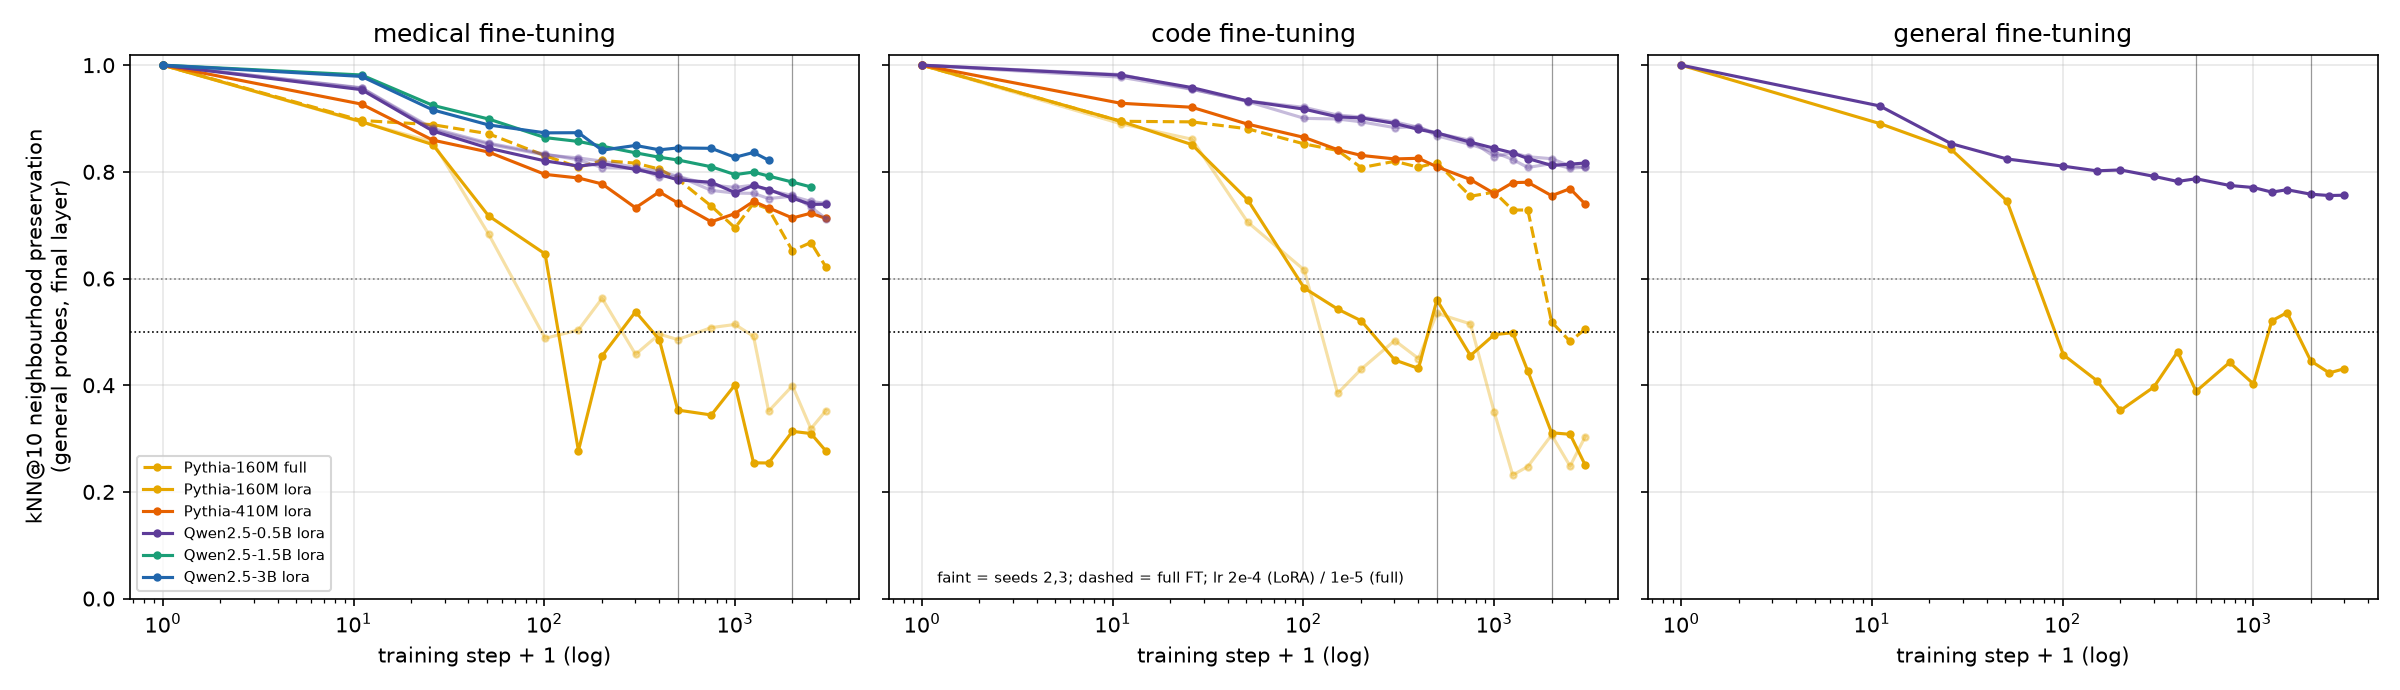
\includegraphics[width=0.98\linewidth]{figures/fig1_preservation_trajectories.png}
    \caption{\pres of 1,000 general-text probes (final layer) against training step for medical, code, and general fine-tuning. Faint lines are additional seeds; dashed lines are full fine-tuning of \pythiaS. Most of the loss happens in the first $\sim$100 steps. Larger Qwen models drift less, but only \pythiaS under LoRA falls below 0.5 (dotted line) with the standard recipe, and all those runs diverged in in-domain loss.}
    \label{fig:trajectories}
\end{figure}

\section{Related Work}
\label{sec:related}

\para{Representation change under fine-tuning.} \citet{merchant2020happens} showed that fine-tuning BERT mostly changes the upper layers and leaves lower layers close to the pretrained model. Representation similarity is usually measured globally, with SVCCA~\citep{raghu2017svcca} or centred kernel alignment~\citep{kornblith2019similarity}. Global measures can hide large changes in local structure, because a near-rotation of the space keeps CKA high while neighbours change. We therefore focus on kNN neighbourhood preservation, a local measure common in dimensionality-reduction evaluation~\citep{venna2006local}, and report CKA alongside it. Unlike earlier end-of-training comparisons, we follow the full trajectory over 17 checkpoints.

\para{Anisotropy of contextual embeddings.} Contextual representations occupy a narrow cone~\citep{ethayarajh2019contextual}, and removing dominant directions improves static embeddings~\citep{mu2018allbutthetop}. \citet{rudman2022isoscore} proposed IsoScore to measure how uniformly a space uses its dimensions. These works describe the isotropy of a trained model. We ask whether fine-tuning moves isotropy in a consistent direction, and find that it does not.

\para{Forgetting in language-model fine-tuning.} Catastrophic forgetting has been studied since early connectionist work~\citep{mccloskey1989catastrophic,kirkpatrick2017overcoming}. For LLMs, \citet{luo2023empirical} measured forgetting during continual instruction tuning, \citet{kalajdzievski2024scaling} fitted scaling laws relating forgetting to fine-tuning loss and parameter count, and \citet{biderman2024lora} showed that LoRA~\citep{hu2022lora} learns less and forgets less than full fine-tuning. Our learning-rate and full fine-tuning ablations agree that update size, not only scale, sets how much is lost. We add a link between local geometry and item-level forgetting, and show that the geometry-to-forgetting mapping differs across model families.

\para{Domain distance and transfer.} Domain-adaptive pretraining work~\citep{gururangan2020dont} uses vocabulary overlap to describe how far a domain is from pretraining data. We test whether this distance predicts how much general-text geometry fine-tuning preserves, and find the opposite of the intuitive prediction.

\section{Method}
\label{sec:method}

\subsection{Measuring geometric drift}

Let $f_t$ be the model after $t$ fine-tuning steps and $\{x_i\}_{i=1}^{N}$ a fixed probe set. We represent each probe by $\vh_i^t$, the mean of the hidden states at positions $\geq 1$ of a given layer. We skip position 0 because it acts as an attention sink. We use the final (post-norm) layer as the primary view and the middle layer as a robustness check. All metrics compare step $t$ with step 0.

\para{kNN preservation.} Let $N_k^t(i)$ be the $k$ nearest neighbours of probe $i$ under cosine similarity at step $t$. Preservation is
\begin{equation}
    P_k(t) = \frac{1}{N}\sum_{i=1}^{N} \frac{|N_k^0(i)\cap N_k^t(i)|}{k}.
\end{equation}
$P_k(t)=1$ means every probe keeps all its neighbours. Our primary metric is $P_{10}$; we also report $k\in\{5,20\}$ and a mean-centred variant that removes the effect of a shared offset.

\para{Global similarity and isotropy.} We compute linear CKA~\citep{kornblith2019similarity} between $\mH^0$ and $\mH^t$. We measure isotropy in three ways: mean pairwise cosine (higher means more anisotropic), IsoScore~\citep{rudman2022isoscore}, and effective rank, the exponential of the entropy of the normalised covariance eigenvalues.

\para{Forgetting.} General knowledge (\gk) is the pooled accuracy on 1,070 items: 570 \mmlu questions~\citep{hendrycks2021measuring} (10 per subject, 0-shot, argmax over the log-probabilities of `` A''--`` D'') and 500 \arce test questions~\citep{clark2018think} (length-normalised accuracy). We also measure per-token NLL on $64\times512$ held-out tokens of \wikitext~\citep{merity2016pointer} and of the in-domain corpus.

\subsection{Models and training}

We use base checkpoints from two families: \qwenS, \qwenM, \qwenL~\citep{qwen2024qwen25}, which share a tokenizer and pretraining corpus, and \pythiaS and \pythiaM~\citep{biderman2023pythia}, trained on the Pile. The standard recipe is identical for every size, so that steps are comparable. It applies LoRA~\citep{hu2022lora} (rank 64, $\alpha=128$, no dropout) to every linear layer and trains with AdamW ($\beta=(0.9,0.95)$, lr 2e-4, 50 warm-up steps then constant, gradient clipping at 1.0, no weight decay). Each step uses a batch of $4\times512$ tokens, so 3,000 steps cover 6.1M tokens. Weights are in bf16 with gradient checkpointing.

\para{Ablations.} To separate model size from update size, we train \qwenS with LoRA at lr 5e-4 and 1e-3, and \pythiaS with full fine-tuning (fp32 master weights, bf16 autocast, lr 1e-5). We run three seeds for \qwenS medical and code, two for \pythiaS medical and code, and one elsewhere; the seed sets document order and LoRA initialisation. In total we analyse 22 runs (\tabref{tab:h1}).

\subsection{Data}

\para{Fine-tuning corpora.} Medical: 40k synthetic clinical notes from \asclepius~\citep{kweon2024publicly}. Code: 30k Python files from \codeparrot-clean-valid (800--20k characters, not auto-generated). General (control): \wikitext training paragraphs. The control separates the effect of being fine-tuned at all from the effect of domain shift. Texts are joined with \eos and cut into 512-token chunks.

\para{Probes.} The primary probe set has 1,000 \wikitext test and validation paragraphs truncated to 128 tokens. Secondary sets have 300 held-out medical and 300 held-out code documents. All probe and evaluation data are disjoint from training data.

\para{Vocabulary overlap.} To test the premise of H4, we compare the Qwen-token unigram distribution of $\sim$2M tokens per corpus with \wikitext, using Jensen--Shannon divergence (JSD), the token mass inside the top 10k \wikitext tokens, and word-type coverage.

\subsection{Evaluation protocol and statistics}

We evaluate 17 checkpoints, at steps 0, 10, 25, 50, 100, 150, 200, 300, 400, 500, 750, 1,000, 1,250, 1,500, 2,000, 2,500, and 3,000. We estimate threshold-crossing steps by linear interpolation in $\log(1+t)$. For forgetting, we run an exact McNemar test on the 1,070 items, comparing each checkpoint with step 0. For H2 we compute Spearman correlations with step and count monotonicity violations. For H3 we compare checkpoints above and below preservation 0.6 with a Mann--Whitney U test, and report Spearman correlations. For H4 we use a paired Wilcoxon test over checkpoints matched on model, method, learning rate, seed, and step.

\para{Training health.} We label a run as \emph{learned} if its final in-domain NLL is more than 0.05 nats below the step-0 value, \emph{diverged} if it is more than 0.25 nats above, and \emph{no gain} otherwise. This label turns out to be central to interpreting H1.

\para{Compute.} All runs used 4 shared RTX A6000 GPUs, usually with 2--6\,GB free per GPU. A \pythiaS run took 7--10 minutes and a \qwenS run 20--26 minutes. The \qwenM and \qwenL medical runs were stopped at steps 2,500 and 1,500 because of GPU contention. A 7B run started but ran out of memory when another job on the same GPU grew (\secref{sec:limitations}).

\section{Results}
\label{sec:results}

\subsection{H1: Bigger models drift less, but the recipe sets the speed}
\label{sec:h1}

\begin{table}[t]
    \centering
    \caption{\pres of general-text probes (final layer) by step. Values are means over seeds; the standard deviation across the three \qwenS seeds is $\leq 0.016$. ``Cross'' is the interpolated step at which preservation first falls below 0.5. ``Health'' compares final with step-0 held-out in-domain NLL. Every run that ends below 0.5 is labelled \emph{diverged}. Highest preservation per column among standard-recipe medical runs in \textbf{bold}.}
    \label{tab:h1}
    \resizebox{\textwidth}{!}{%
    \begin{tabular}{@{}lllccccccll@{}}
        \toprule
        \textbf{Model} & \textbf{Recipe} & \textbf{Domain} & \textbf{10} & \textbf{100} & \textbf{500} & \textbf{1000} & \textbf{2000} & \textbf{3000} & \textbf{Cross} & \textbf{Health} \\
        \midrule
        \pythiaS (2 seeds) & LoRA 2e-4 & medical & 0.89 & 0.57 & 0.42 & 0.46 & 0.36 & 0.31 & $\sim$96--117 & diverged \\
        \pythiaS (2 seeds) & LoRA 2e-4 & code & 0.89 & 0.60 & 0.55 & 0.42 & 0.31 & 0.28 & $\sim$123--224 & diverged \\
        \pythiaS & LoRA 2e-4 & general & 0.89 & 0.46 & 0.39 & 0.40 & 0.45 & 0.43 & $\sim$90 & diverged \\
        \pythiaS & full 1e-5 & medical & 0.90 & 0.83 & 0.79 & 0.70 & 0.65 & 0.62 & never & learned \\
        \pythiaS & full 1e-5 & code & 0.90 & 0.85 & 0.82 & 0.76 & 0.52 & 0.51 & ($\sim$2,240) & no gain \\
        \pythiaM & LoRA 2e-4 & medical & 0.93 & 0.80 & 0.74 & 0.72 & 0.71 & 0.71 & never & learned \\
        \pythiaM & LoRA 2e-4 & code & 0.93 & 0.87 & 0.81 & 0.76 & 0.76 & 0.74 & never & diverged \\
        \midrule
        \qwenS (3 seeds) & LoRA 2e-4 & medical & 0.96 & 0.83 & 0.79 & 0.76 & 0.75 & 0.73 & never & learned \\
        \qwenS (3 seeds) & LoRA 2e-4 & code & 0.98 & 0.91 & 0.87 & 0.84 & 0.82 & 0.81 & never & no gain \\
        \qwenS & LoRA 2e-4 & general & 0.92 & 0.81 & 0.79 & 0.77 & 0.76 & 0.76 & never & learned \\
        \qwenS & LoRA 5e-4 & medical & 0.91 & 0.78 & 0.70 & 0.65 & 0.58 & 0.57 & never & learned \\
        \qwenS & LoRA 5e-4 & code & 0.96 & 0.86 & 0.77 & 0.73 & 0.66 & 0.63 & never & diverged \\
        \qwenS & LoRA 1e-3 & medical & 0.88 & 0.71 & 0.43 & 0.35 & 0.25 & 0.22 & $\sim$420 & diverged \\
        \qwenS & LoRA 1e-3 & code & 0.95 & 0.78 & 0.50 & 0.37 & 0.28 & 0.27 & $\sim$500 & diverged \\
        \qwenM & LoRA 2e-4 & medical & {\bf 0.98} & 0.86 & 0.82 & 0.80 & {\bf 0.78} & (0.77 @2,500) & never & learned \\
        \qwenL & LoRA 2e-4 & medical & {\bf 0.98} & {\bf 0.87} & {\bf 0.85} & {\bf 0.83} & -- & (0.82 @1,500) & never & learned \\
        \bottomrule
    \end{tabular}
    }
\end{table}


\Tabref{tab:h1} and \figref{fig:size_recipe} show \pres of the general-text probes over training.

\para{Scale helps at matched steps.} Within each family, preservation rises with size at every matched step (\figref{fig:size_recipe}, left). After 1,000 medical steps, Qwen preservation is 0.76, 0.80, and 0.83 for 0.5B, 1.5B, and 3B. \pythiaM is far more stable than \pythiaS (0.74 \versus 0.42 at step 500). The direction of H1 therefore holds.

\para{But sub-1B is not enough for collapse.} \qwenS (494M parameters) never falls below 0.71 in 3,000 steps under the standard recipe. Only \pythiaS crosses 0.5 within 500 steps, at roughly steps 90--220.

\para{The learning rate matters more than size.} Raising the LoRA learning rate on \qwenS from 2e-4 to 5e-4 to 1e-3 lowers final medical preservation from 0.73 to 0.57 to 0.22 (\figref{fig:size_recipe}, right). At lr 1e-3, \qwenS crosses 0.5 at steps $\sim$420--500, which matches the H1 prediction. For \pythiaS, full fine-tuning at lr 1e-5 keeps 0.62 after 3,000 medical steps, while LoRA at lr 2e-4 falls to 0.31. A fivefold change in learning rate on one model moves final preservation by 0.51 (0.73 $\rightarrow$ 0.22), while a sixfold change in Qwen size moves step-500 preservation by only 0.06 (0.79 $\rightarrow$ 0.85).

\para{Collapse goes together with failed optimisation.} All seven runs that end below 0.5 have \emph{rising} held-out in-domain NLL. \pythiaS LoRA runs lose 0.5--2.1 nats in every domain, including on \wikitext itself, and \qwenS at lr 1e-3 loses 0.4 (medical) and 1.5 (code) nats. Runs that actually learn their domain end between 0.57 and 0.82. Fast loss of pretraining geometry in these runs is therefore a symptom of destructive optimisation, not of successful specialisation.

\para{Most drift happens early.} In all runs, most of the change happens in the first $\sim$100 steps. After that, curves decline slowly on a log-step axis (\figref{fig:trajectories}).

\para{Fine-tuning itself, not the domain, causes most drift.} The \wikitext control drifts about as much as domain fine-tuning: \qwenS ends at 0.76 after general fine-tuning \versus 0.73 after medical fine-tuning.

\para{Robustness.} $k=5$ and $k=20$ give the same ordering of runs; $k=20$ values are 0.01--0.05 higher. The mean-centred variant is on average 0.024 higher (at most 0.12) with the same ordering. The middle layer is usually somewhat more stable (median $+0.04$) and shows the same pattern.

\begin{figure}[t]
    \centering
    \begin{subfigure}[b]{0.39\textwidth}
        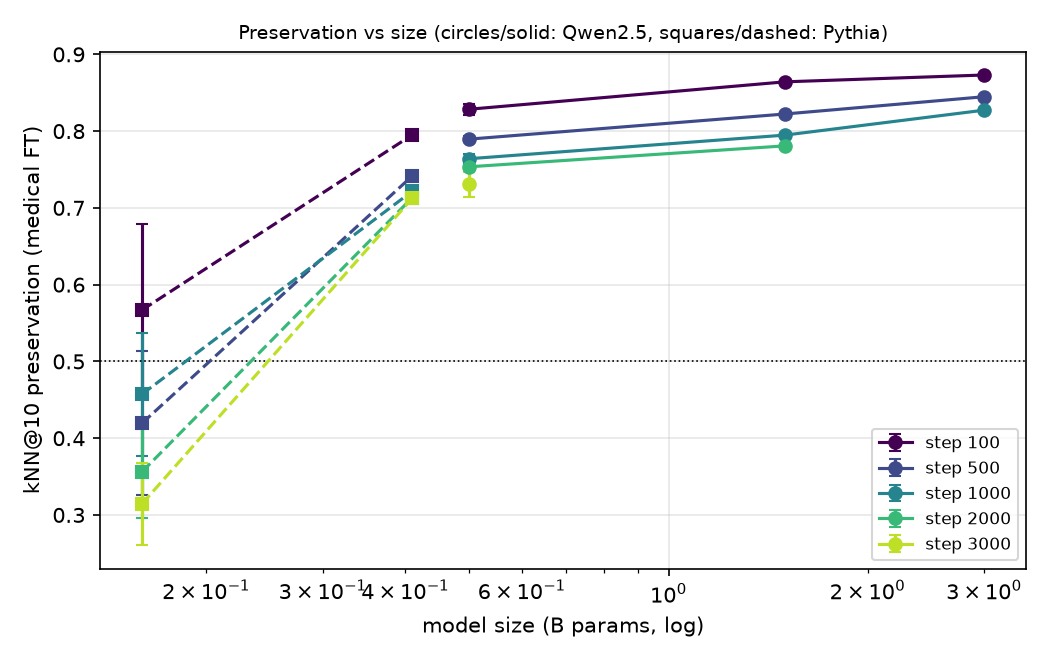
\includegraphics[width=\textwidth]{figures/fig5_preservation_vs_size.png}
        \caption{Preservation \versus model size}
        \label{fig:size}
    \end{subfigure}
    \hfill
    \begin{subfigure}[b]{0.59\textwidth}
        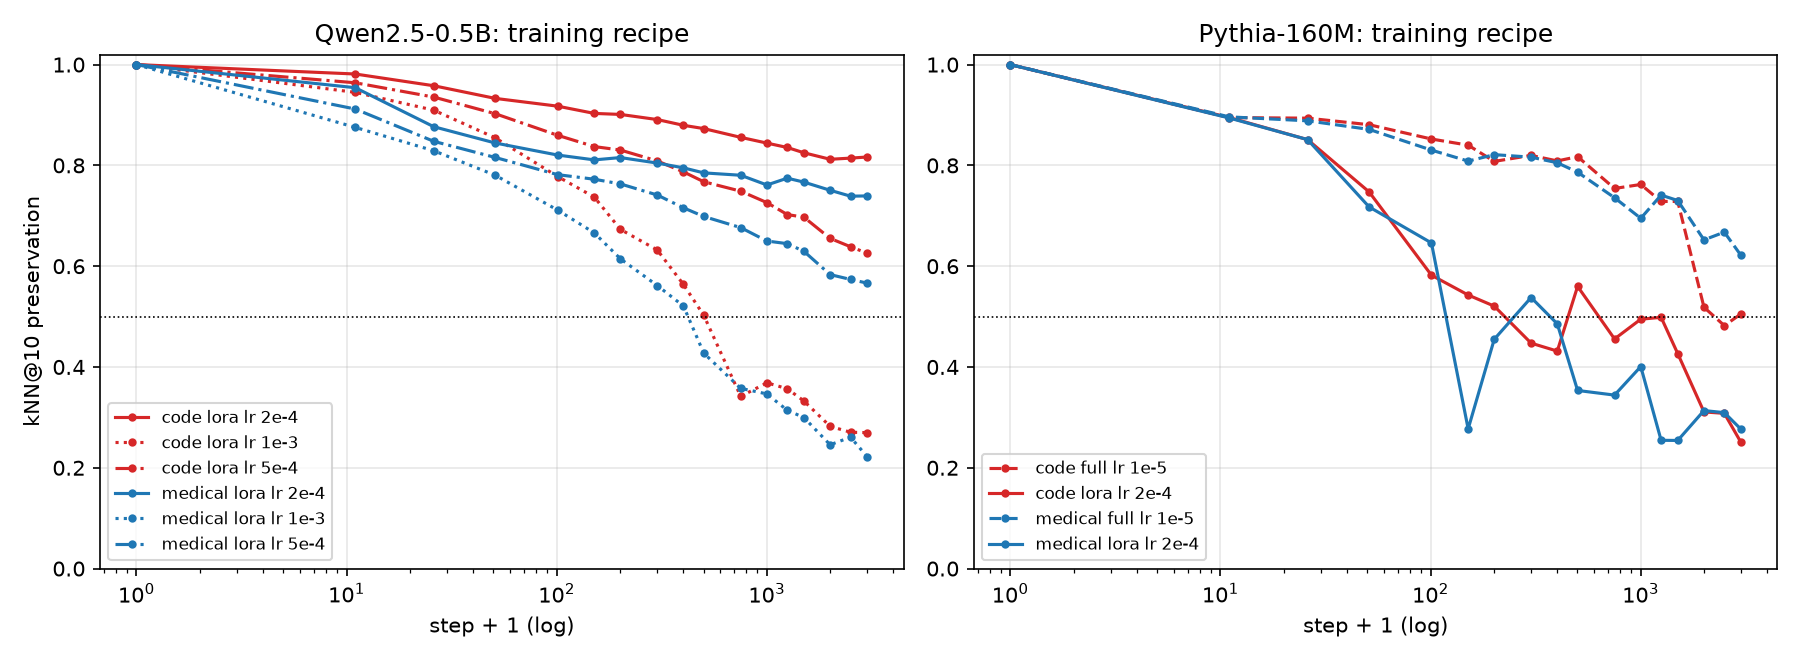
\includegraphics[width=\textwidth]{figures/fig6_recipe_ablation.png}
        \caption{Recipe ablations}
        \label{fig:recipe}
    \end{subfigure}
    \caption{\textbf{(a)} Medical fine-tuning, standard LoRA recipe: preservation grows with size at each step within each family (squares: Pythia; circles: Qwen2.5; error bars over seeds). \textbf{(b)} Changing the recipe on a single model moves preservation much more than size does. For \qwenS, lr 1e-3 drives preservation to $\sim$0.25, and for \pythiaS, full fine-tuning at lr 1e-5 (dashed) drifts far less than LoRA at 2e-4.}
    \label{fig:size_recipe}
\end{figure}

\subsection{H2: Isotropy does not fall monotonically}
\label{sec:h2}

\begin{table}[t]
    \centering
    \small
    \caption{Isotropy change over 22 runs (final layer, general probes). No run moves monotonically toward anisotropy on any measure, and the median net change is a few percent.}
    \label{tab:h2}
    \begin{tabular}{@{}lccc@{}}
        \toprule
        \textbf{Measure} & \textbf{Monotone} & \textbf{Net more anisotropic} & \textbf{Median change} \\
        \midrule
        Mean pairwise cosine ($\uparrow$ anisotropic) & 0 / 22 & 14 / 22 & $+2.3\%$ \\
        \isoscore ($\downarrow$ anisotropic) & 0 / 22 & 18 / 22 & $-8.3\%$ \\
        Effective rank ($\downarrow$ anisotropic) & 0 / 22 & 17 / 22 & $-5.7\%$ \\
        \bottomrule
    \end{tabular}
\end{table}

\Tabref{tab:h2} and \figref{fig:isotropy} summarise isotropy. Most runs end slightly more anisotropic than they started, but none gets there monotonically. \pythiaS LoRA runs first become much \emph{more} isotropic (\isoscore up to 1.6$\times$ its step-0 value at steps 100--500) and then fall back. Meanwhile, local neighbourhood structure loses 20--80\% of its overlap. Fine-tuning reshuffles neighbours long before it changes the global spectral shape of the space. {\bf H2 is not supported}, and global isotropy is a weak drift signal.

\begin{figure}[t]
    \centering
    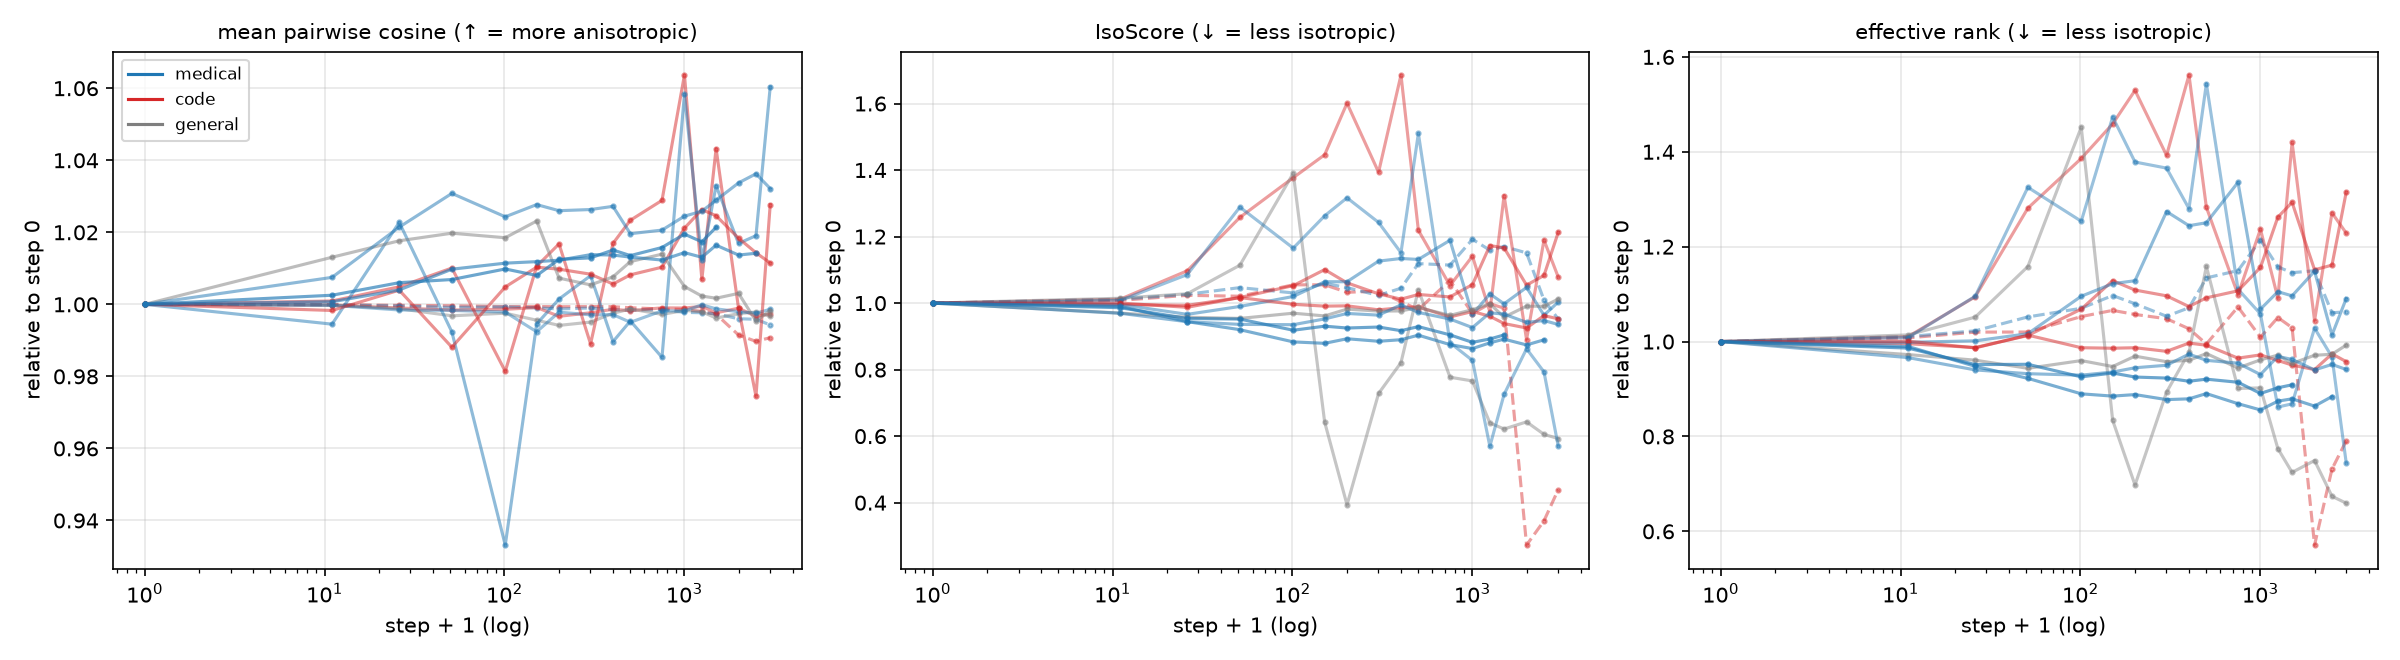
\includegraphics[width=0.95\linewidth]{figures/fig2_isotropy.png}
    \caption{Three isotropy measures relative to step 0 for all runs (blue: medical; red: code; grey: general; dashed: full fine-tuning). Trajectories are noisy and non-monotone, and net changes are small compared with the loss of neighbourhood structure in \figref{fig:trajectories}.}
    \label{fig:isotropy}
\end{figure}

\subsection{H3: Preservation tracks forgetting, but there is no 0.6 threshold}
\label{sec:h3}

\para{Overall association.} Across all 348 non-zero checkpoints, lower preservation goes with more forgetting. Checkpoints with preservation $\geq 0.6$ ($n=260$) lose 2.7\pp \gk accuracy on average, and 39\% show a significant decline. Checkpoints below 0.6 ($n=88$) lose 9.2\pp, and 82\% show a significant decline (Mann--Whitney $p=5\times10^{-12}$). Spearman $\rho$ between preservation and $\Delta$\gk is 0.69, and between preservation and $\Delta$\wikitext NLL it is $-0.90$.

\para{Forgetting starts well above 0.6.} \Tabref{tab:h3_onset} lists the first checkpoint with a significant \gk decline for each run. In 16 of the 21 runs with a detected decline, forgetting begins while preservation is still $\geq 0.6$, usually at 0.77--0.90. \qwenS loses 8.8\pp \gk after 3,000 medical steps and 9.9\pp after 3,000 \wikitext steps, while its preservation stays $\geq 0.71$. At lr 5e-4 it loses 11.7\pp by step 500, at preservation 0.70. The only runs that start forgetting below 0.6 are the diverged \pythiaS LoRA runs.

\begin{table}[t]
    \centering
    \small
    \caption{First checkpoint with a significant drop in general-knowledge accuracy (McNemar $p<.05$ against step 0) and the preservation at that point. Only the \pythiaS LoRA runs, all of which diverged, start forgetting below the hypothesised 0.6 threshold.}
    \label{tab:h3_onset}
    \begin{tabular}{@{}lcc@{}}
        \toprule
        \textbf{Run} & \textbf{Onset step} & \textbf{Preservation at onset} \\
        \midrule
        \qwenS medical (seeds 1/2/3) & 500 / 400 / 750 & 0.79 / 0.80 / 0.77 \\
        \qwenS general & 100 & 0.81 \\
        \qwenS lr 5e-4 (medical / code) & 50 / 300 & 0.82 / 0.81 \\
        \qwenS lr 1e-3 (medical / code) & 50 / 100 & 0.78 / 0.78 \\
        \qwenM medical & 50 & 0.90 \\
        \qwenL medical & 200 & 0.84 \\
        \pythiaM (medical / code) & 150 / 500 & 0.79 / 0.81 \\
        \pythiaS LoRA (5 runs) & 100--300 & 0.43--0.50 \\
        \pythiaS full FT (code / medical) & 1,500 / 2,500 & 0.73 / 0.67 \\
        \bottomrule
    \end{tabular}
\end{table}


\para{The mapping differs across families.} At preservation $\approx 0.25$, \qwenS (lr 1e-3) has lost 30\pp \gk, while \pythiaS has lost only $\sim$4\pp (\figref{fig:forgetting}, left). Part of this gap comes from Pythia's \mmlu accuracy being at chance ($\sim$23\%), so its \gk signal comes only from \arce. Still, the same preservation value means very different amounts of benchmark damage in the two families.

\para{General-text perplexity is the exception.} The relation between preservation and $\Delta$\wikitext NLL is tight and nearly the same for all models (\figref{fig:forgetting}, right). Losing neighbourhood structure on general text goes together with losing general-text language modelling. The one exception is the \wikitext control, where NLL improves while preservation drops. {\bf H3 is not supported}: preservation is associated with forgetting, but there is no onset at 0.6. For Qwen models, accuracy-based forgetting begins around 0.8.

\begin{figure}[t]
    \centering
    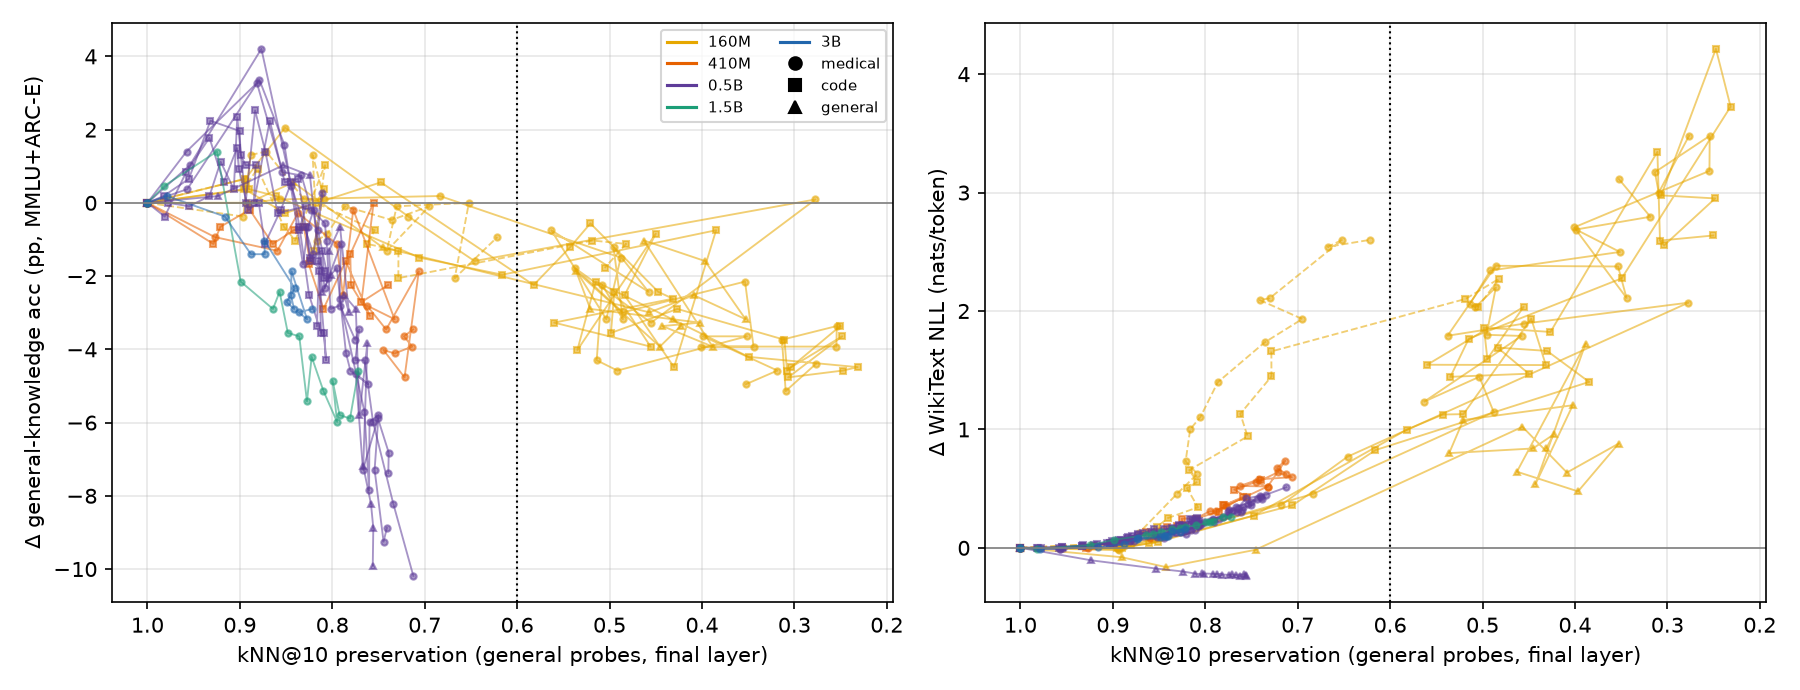
\includegraphics[width=0.95\linewidth]{figures/fig3_preservation_vs_forgetting.png}
    \caption{Preservation against forgetting for every checkpoint (colour: model; marker: domain; dashed: full fine-tuning). \textbf{Left:} change in \gk accuracy. Qwen models (purple, green, blue) lose up to 10\pp while preservation is still above 0.7, whereas \pythiaS (yellow) loses only a few points at 0.3. The dotted line marks the hypothesised 0.6 threshold. \textbf{Right:} change in \wikitext NLL. The relation is tight and shared across models; the lower branch is the \wikitext control run.}
    \label{fig:forgetting}
\end{figure}

\subsection{H4: Code preserves more general geometry than medical text}
\label{sec:h4}

\begin{table}[t]
    \centering
    \small
    \caption{Medical \versus code fine-tuning. \textbf{Top:} paired differences over 144 checkpoints matched on model, recipe, seed, and step (Wilcoxon signed-rank). Negative preservation differences mean medical preserves \emph{less}. \textbf{Bottom:} vocabulary overlap of each corpus with \wikitext ($\sim$2M Qwen tokens each). Medical text is much closer to general text, yet it preserves less general-text geometry.}
    \label{tab:h4}
    \begin{tabular}{@{}lcc@{}}
        \toprule
        \textbf{Paired comparison} & \textbf{Medical $-$ code} & \textbf{$p$} \\
        \midrule
        \pres & $-0.043$ (medical higher at 17\%) & $3\times10^{-12}$ \\
        Centred \pres & $-0.044$ & $3\times10^{-14}$ \\
        CKA & $-0.011$ & $2\times10^{-11}$ \\
        $\Delta$ \gk accuracy & $-1.9$\pp (medical forgets more) & $3\times10^{-10}$ \\
        $\Delta$ \wikitext NLL & $+0.21$ nats (medical forgets more) & $9\times10^{-18}$ \\
        \midrule
        \textbf{Corpus overlap with \wikitext} & \textbf{Medical} & \textbf{Code} \\
        \midrule
        Unigram JSD (bits, $\downarrow$ closer) & {\bf 0.45} & 0.63 \\
        Token mass in top-10k \wikitext tokens & {\bf 67\%} & 36\% \\
        Word-type coverage & {\bf 90\%} & 80\% \\
        \bottomrule
    \end{tabular}
\end{table}


\para{The premise holds; the prediction fails.} Clinical notes are much closer to \wikitext than Python code is (JSD 0.45 \versus 0.63 bits; \tabref{tab:h4}). Yet over 144 matched checkpoints, medical fine-tuning preserves \emph{less} general-text geometry than code ($-0.043$, medical higher at only 17\% of checkpoints, $p=3\times10^{-12}$). Medical fine-tuning also causes more forgetting: 1.9\pp more \gk loss and 0.21 nats more \wikitext NLL increase. All three \qwenS seeds agree (final preservation 0.74 / 0.71 / 0.74 for medical \versus 0.82 / 0.81 / 0.81 for code), as do \qwenS at lr 5e-4 (0.57 \versus 0.63) and 1e-3 (0.22 \versus 0.27), and \pythiaM (0.71 \versus 0.74). Only \pythiaS follows H4's direction (LoRA: 0.28 / 0.35 \versus 0.25 / 0.30; full fine-tuning: 0.62 \versus 0.51), and its LoRA runs diverged in both domains.

\para{Two possible explanations.} The first is \emph{interference}. Clinical English uses the same tokens and features as general English, so adapting to it rewrites features that general text depends on, while code lives in a more separate region of the space. The second is \emph{amount of change}. The base models already model this Python corpus well. Under the standard recipe, code fine-tuning gave no in-domain gain for \qwenS (held-out NLL 1.58 $\rightarrow$ 1.68), while medical fine-tuning really adapted the model (2.34 $\rightarrow$ 1.98). Small, noise-like updates should move the geometry less. Our design cannot separate these two explanations, because the domain contrast is confounded with how much there is to learn. Either way, {\bf H4 is not supported}, and vocabulary overlap does not predict geometric preservation here. As expected for real domain adaptation, under medical fine-tuning the medical probes move the most (\qwenS: 0.64 for medical probes \versus 0.74 for general probes).

\section{Discussion}
\label{sec:discussion}

{\bf Is collapse speed a property of model size?} Only partly. Within a family and a fixed recipe, larger models keep more geometry and forget less, which agrees with prior reports that larger models forget less~\citep{kalajdzievski2024scaling}. But the number of steps until preservation falls below 50\% is not a size constant. It depends mainly on update size (learning rate, LoRA \versus full fine-tuning) and on whether optimisation stays healthy. Under the standard recipe, healthy runs of models from 410M to 3B level off at 0.7--0.85 on a log-step axis. Extrapolating, a 7B model would very likely stay above 0.5 past 2,000 steps. That would make H1's 7B clause true but uninformative, since a 0.5B model already behaves this way. We did not measure 7B.

{\bf What is preservation good for?} We see three uses and one non-use.
\begin{itemize}[leftmargin=*,itemsep=0pt,topsep=0pt]
    \item It is a cheap, label-free proxy for damage to general-text language modelling, and its relation to $\Delta$NLL is nearly the same across models ($\rho=-0.90$).
    \item A sharp early drop (\eg below $\sim$0.6 within a few hundred steps) is a strong sign of over-aggressive or unstable fine-tuning. Every such run in our study also had rising in-domain loss.
    \item Because most drift happens in the first $\sim$100 steps, a monitor can flag a bad learning rate very early in training.
    \item It is not a calibrated alarm for benchmark forgetting. Qwen models lose \mmlu and \arce accuracy at preservation 0.8--0.9, and part of the \mmlu loss reflects losing the multiple-choice answer \emph{format}: plain language-model training on \wikitext costs \qwenS 11\pp on \mmlu. A practical monitor should combine the \emph{rate} of preservation loss with a family-specific calibration, or track probe-set NLL directly.
\end{itemize}

{\bf Why do global and local geometry disagree?} Fine-tuning reorders local neighbourhoods long before it changes the global spectrum of the space. Isotropy summarises the covariance of all probes, so it stays within a few percent while 20--80\% of neighbour overlap is lost. Global isotropy statistics are therefore poor drift indicators.

{\bf Surprises.} Three results ran against our expectations. First, in-distribution fine-tuning on \wikitext drifts about as much as domain fine-tuning and causes the largest \mmlu loss for \qwenS. Second, \pythiaS diverges under LoRA at lr 2e-4 in every domain, while full fine-tuning at lr 1e-5 learns stably. Third, fine-tuning Qwen2.5 on Python barely changes in-domain loss, because these base models are already strong on code.

\subsection{Limitations}
\label{sec:limitations}

\para{Scale coverage.} We have no 7B results. A 7B run started on the only large GPU slice but ran out of memory when another user's job grew; at the measured $\sim$7\,s per step plus 8.5 minutes per evaluation, it could not have finished. The \qwenM and \qwenL medical runs stop at 2,500 and 1,500 steps, and we have no 1.5B or 3B code runs, so H4 is tested only at $\leq$0.5B.

\para{Recipe coverage.} Each size uses one standard recipe, and the learning-rate and full fine-tuning ablations cover one model each. In practice larger models often get smaller learning rates, which would reduce their drift further.

\para{Domain confound.} Code fine-tuning did not lower in-domain loss, so the domain contrast is confounded with the amount of adaptation. A design that matches in-domain loss reduction across domains would separate the two explanations in \secref{sec:h4}.

\para{Seeds and noise.} Only \qwenS (three seeds) and \pythiaS (two seeds) medical and code runs are replicated. Seed variation is small for Qwen ($\leq 0.016$) but reaches $\sim$0.09 for the diverging \pythiaS runs. A single \gk estimate on 1,070 items has about $\pm$2.5\pp sampling noise, which paired McNemar tests reduce but do not remove. \mmlu is at chance for Pythia.

\para{Probes and proxies.} We use mean-pooled 128-token \wikitext probes. Token-level or static-embedding neighbourhoods may behave differently, and under LoRA the input embedding matrix is frozen. \wikitext stands in for pretraining data, and the medical corpus consists of LLM-written synthetic notes rather than real clinical text.

\para{Broader impact.} A cheap geometric monitor could reduce the compute spent on evaluation during fine-tuning. Our results warn against relying on one fixed threshold: a monitor tuned on one model family could miss substantial forgetting in another, which matters when fine-tuned models are deployed in sensitive domains such as medicine.

\section{Conclusion}
\label{sec:conclusion}

We tracked how fine-tuning reshapes the local neighbourhood structure of language-model representations across 22 runs, five model sizes, three domains, and 17 checkpoints. Fine-tuning changes neighbourhoods quickly, mostly within the first $\sim$100 steps, and larger models change less at matched steps. All four specific hypotheses fail. Collapse below 50\% depends on the learning rate and on training stability more than on a sub-1B \versus 7B split. Isotropy never declines monotonically. Benchmark forgetting begins while preservation is still around 0.8, not at 0.6. Code fine-tuning, not medical, preserves more general-text geometry for most models, despite lower vocabulary overlap.

{\bf Takeaway:} kNN preservation is a cheap proxy for damage to general language modelling and a reliable sign of unstable fine-tuning. It is not a universal forgetting threshold.

Future work should run 7B models and complete the 1.5B and 3B code runs on dedicated hardware, fit crossing time as a function of update norm with a learning-rate $\times$ size grid, and compare domains matched on in-domain loss reduction. A lead-time analysis would show whether probe-set NLL, CKA, or kNN preservation gives the earliest warning. Replay or L2-SP regularisation~\citep{li2018explicit} could test whether preservation can be decoupled from forgetting.


\bibliography{references}

\newpage
\appendix
\section{Additional Experimental Details}
\label{app:details}

\para{LoRA target modules.} For Qwen2.5 we adapt \texttt{q\_proj}, \texttt{k\_proj}, \texttt{v\_proj}, \texttt{o\_proj}, \texttt{gate\_proj}, \texttt{up\_proj}, and \texttt{down\_proj}. For Pythia we adapt \texttt{query\_key\_value}, \texttt{dense}, \texttt{dense\_h\_to\_4h}, and \texttt{dense\_4h\_to\_h}.

\para{Memory.} To fit training into 2--5\,GB GPU slices, the loss is computed over 256-token chunks with recomputation, together with gradient checkpointing.

\para{Corpora.} Each run uses a seeded prefix of $\sim$6.1M tokens from its corpus. Code files are 800--20k characters long and filtered to exclude auto-generated files.

\para{Held-out in-domain NLL (nats per token, step 0 $\rightarrow$ step 3,000).}

\begin{table}[h]
    \centering
    \small
    \caption{Held-out in-domain NLL before and after fine-tuning under the standard recipe. Code fine-tuning gives no gain for \qwenS, and \pythiaS LoRA diverges in both domains.}
    \label{tab:nll}
    \begin{tabular}{@{}lcc@{}}
        \toprule
        \textbf{Model} & \textbf{Code} & \textbf{Medical} \\
        \midrule
        \qwenS (lr 2e-4) & 1.58 $\rightarrow$ 1.68 (no gain) & 2.34 $\rightarrow$ {\bf 1.98} (learned) \\
        \pythiaM & 1.55 $\rightarrow$ 1.83 & 2.34 $\rightarrow$ 2.08 \\
        \pythiaS LoRA & 2.18 $\rightarrow$ 4.24 (diverged) & 3.15 $\rightarrow$ 3.79 (diverged) \\
        \bottomrule
    \end{tabular}
\end{table}

\para{Word-type coverage and floors.} As a floor for the vocabulary-overlap measures, a split-half comparison of \wikitext with itself gives JSD 0.01 bits, 91\% token mass in the top-10k tokens, and 97\% word-type coverage.

\para{Domain comparison figure.} \Figref{fig:domain} overlays all seed-1 runs by domain.

\begin{figure}[h]
    \centering
    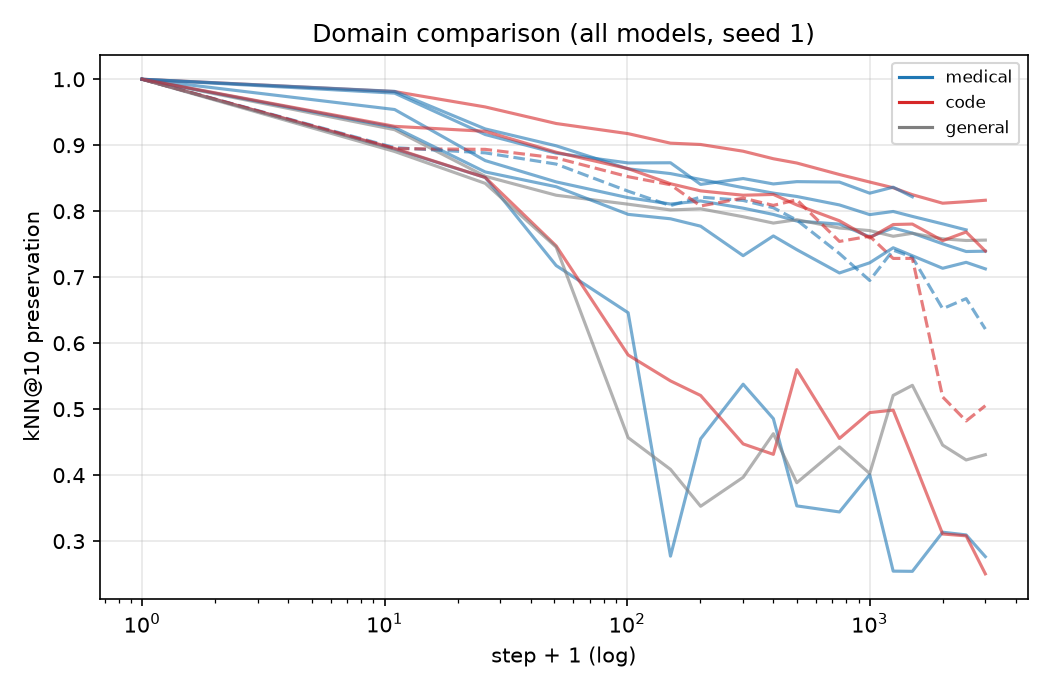
\includegraphics[width=0.6\linewidth]{figures/fig4_domain_comparison.png}
    \caption{\pres for all models (seed 1), coloured by fine-tuning domain. Among the stable runs at the top, code (red) usually lies above medical (blue). The low cluster is the diverging \pythiaS LoRA runs.}
    \label{fig:domain}
\end{figure}

\para{Software.} Python 3.12.12, torch 2.14.1, transformers 5.20.2, peft 0.21.2, numpy 2.5.4, scipy 1.18.1, pandas 3.1.0. No external APIs were used.


\end{document}
